% uklad dokumentu
	\documentclass{article}
	\usepackage{xparse}
	\usepackage[margin=1.5cm]{geometry}
    \usepackage{enumerate} 
	\frenchspacing
    \linespread{1.0}
    \setlength{\parindent}{0pt}

% jezyk polski
	\usepackage[T1]{fontenc}
	\usepackage[polish]{babel}
	\usepackage[utf8]{inputenc}
 
% pakiety matematyczne
    \let\lll\undefined
    \usepackage{mathtools}
	\usepackage{amssymb}
    \usepackage{amsthm}
	\usepackage{amsmath}
	\usepackage{amsfonts}
	\usepackage{tikz}
	\usepackage{multirow}

	\usepackage{float}	
	
% pakiety do automatów
	\usetikzlibrary{automata, arrows.meta, positioning, arrows}
	
% wykresiki
	\usepackage{pgfplots}
	\pgfplotsset{compat = newest}
	\usepackage{graphicx}
	\usepackage{subcaption}

    \title{\textbf{Algorytmy Metaheurystyczne\\Tabu w Komiwojażerze}}
    \author{Gabriel Budziński(254609)\\Franciszek Stepek (256310)}
    \date{}
    
    
\begin{document} 
\maketitle

\section*{Przedmowa}
Na samym początku omówimy po krótce użyte algorytmy, oraz zastanowimy się nad ich złożonością obliczeniową, natomiast dalej dopiero przejdziemy do opisu eksperymentów.

\section{Opis eksperymentów}
\subsection{Implementacja}
Algorytmy implementujemy w języku \texttt{C/C++}, odległości między wierzchołkami są przechowywane jako pełne tablice dwuwymiarowe typu \texttt{int}, a trasy są w kontenerach \texttt{vector}, co ułatwia operacje odwracania i mieszania.\\
Korzystaliśmy z kompilatora g++ wraz z użyciem flag -lSDL2 (używanej przy wizualizacji, wraz z odpowiednim dla danego systemu operacyjnego podlinkowania do folderu zawierającego) oraz -lpthread (przy korzystaniu z wielowątkowości)

\subsection{Sprzęt}
Programy były testowane na dwóch maszynach, laptopie \textit{Lenovo} i komputerze stacjonarnym. Obie jednostki są wyposażone w procesor architektury \texttt{x86} marki \texttt{intel} oraz 16GB pamięci RAM.

\subsubsection{Pececik}
Komputer stacjonarny posiada procesor sześciordzeniowy i5-10600K 4,1 GHz (o obniżonym napięciu operacyjnym).
\subsubsection{Lapek}
Laptop posiada procesor czterordzeniowy i7-6700HQ 2,6 GHz

\subsection{Instancje}
\subsubsection{Przykłady TSPLIB}
W części eksperymentów użyto instancji euklidejskiego problemu komiwojażera.

\subsubsection{Instancje losowe}
W celu zwiększenia liczności i dokładności testów spreparowano losowo generowane instancje eukidejskiego problemu komiwojażera.

\subsection{Metodologia/cel}

Testy przeprowadzono za pomocą zaimplementowanych w tym celu funkcji ku jak największej automatyzacji. Dane o przeprowadzonych testach zapisywano do plików tekstowych w formacie CSV, a następnie poddane analizie. Testowanie miało na celu wskazanie mocnych i słabych stron zaimplementowanych heurystyk, jak i ich porównanie.

\subsection{Opis wyników}

\subsection{Wyniki z custom-parameter-tuner}
Zaimplementowany został także masowy test, który miał na celu wynalezienie 'optymalnych' hiperparametrów mając za zbiór testowy 3 instancje (70, 280 oraz 1002 miastowe). Największe różnorodności otrzymano dla instancji z 70 miastami, dla miast 280 można już było zawęzić nieco wyniki, natomiast dla instancji z 1002 miastami różnice okazały się na tyle znaczące, że bez problemu można wyznaczyć najlepsze.
\\\\
Na początku przedstawmy tabelę wynikową dla n = 70. Ale zanim to zrobimy, to dodajmy tylko, że w tabeli 1 zawrzemy jedynie przedstawienie wyników dla otoczenia \textit{Invert}, ponieważ dla pozostałych 2 otoczeń dobór parametrów okazał się praktycznie bez znaczenia po względnie minimalnym odcinku czasu (po około 0.5 sekundy od rozpoczęcia działania każdy z pojedynczych testów ostatecznie zwracał ten sam wynik), gdzie otoczenie \textit{Insert} dało wynik $722$, natomiast \textit{Swap} $756$.

\begin{table}[h!]
	\centering
	\begin{tabular}{c|c|c||c|c|c|c}
	Tabela 1.\\
	Kik Mode & Tabu Size Mode & Enhance Mode & Min & Avg & Max & StDev \\
	\hline
	\textit{Invert} & 7 & Tabu * 2 + 1 & \textbf{675} & \textbf{675} & \textbf{675} & 0 \\
	 &  & Tabu * 10 & \textbf{675} & 692.(3) & 699 & 10 \\
	 &  & Tabu * $\sqrt{Size}$ & \textbf{675} & 687.(6) & 699 & 12.0726964676496 \\
	 &  & Tabu * $log_2(Size)$ & 690 & 696.(8) & 699 & 3.05959329178095 \\
	\cline{2-7}
	 & $\sqrt{Size}$ & Tabu * 2 + 1 & 684 & 694.(3) & 699 & 6.14410286372226 \\
	 &  & Tabu * 10 & \textbf{675} & 693 & 699 & 10.2834819006016 \\
	 &  & Tabu * $\sqrt{Size}$ & \textbf{675} & 691 & 699 & 9.94987437106621 \\
	 &  & Tabu * $log_2(Size)$ & 691 & 696.(7) & 701 & 3.73422608373463 \\
	\cline{2-7}
	 & $log_2(Size)$ & Tabu * 2 + 1 & 686 & 686.(8) & 694 & 2.66666666666666 \\
	 &  & Tabu * 10 & \textbf{675} & 689.(7) & 699 & 9.25712938466584 \\
	 &  & Tabu * $\sqrt{Size}$ & 695 & 697.(6) & 699 & 1.99999999999999 \\
	 &  & Tabu * $log_2(Size)$ & 686 & 695.(4) & 699 & 5.70331287742287 \\
	\hline
	\textit{Insert} & 7 & Tabu * 2 + 1 & 695 & 701.(4) & 707 & 5.05250213040802 \\
	 &  & Tabu * 10 & 696 & 696.(8) & 701 & 1.69148192751537 \\
	 &  & Tabu * $\sqrt{Size}$ & \textbf{\textit{687}} & 696.(4) & 707 & 7.09068246206084 \\
	 &  & Tabu * $log_2(Size)$ & 688 & 691 & 701 & 5.67890834580028 \\
	\cline{2-7}
	 & $\sqrt{Size}$ & Tabu * 2 + 1 & \textbf{\textit{681}} & 694.(3) & 699 & 5.83095189484535 \\
	 &  & Tabu * 10 & 688 & 691.(8) & 708 & 6.97216688778397 \\
	 &  & Tabu * $\sqrt{Size}$ & 688 & 692.(7) & 713 & 8.52610370828576 \\
	 &  & Tabu * $log_2(Size)$ & \textbf{\textit{681}} & 695.(2) & 712 & 11.9035475571127 \\
	\cline{2-7}
	 & $log_2(Size)$ & Tabu * 2 + 1 & 697 & 709.(6) & 716 & 9.5 \\
	 &  & Tabu * 10 & 685 & 692.(7) & 703 & 6.99603062060507 \\
	 &  & Tabu * $\sqrt{Size}$ & \textbf{\textit{681}} & 691.(8) & 703 & 8.22259758902934 \\
	 &  & Tabu * $log_2(Size)$ & 686 & 690.(6) & 696 & 4.76969600708475 \\
\hline
	\textit{Swap} & 7 & Tabu * 2 + 1 & 691 & 694.(3) & 697 & 2.783882181415 \\
	 &  & Tabu * 10 & 691 & 695.(8) & 701 & 4.01386485959743 \\
	 &  & Tabu * $\sqrt{Size}$ & \textbf{\textit{683}} & 692.(3) & 699 & 6.24499799839846 \\
	 &  & Tabu * $log_2(Size)$ & 685 & 691.(8) & 696 & 4.53994615729206 \\
	\cline{2-7}
	 & $\sqrt{Size}$ & Tabu * 2 + 1 & \textbf{\textit{679}} & 683.(7) & 696 & 5.71790559946948 \\
	 &  & Tabu * 10 & 686 & 696.(7) & 701 & 4.86769395550341 \\
	 &  & Tabu * $\sqrt{Size}$ & 686 & 693.(7) & 701 & 6.01618188259331 \\
	 &  & Tabu * $log_2(Size)$ & 686 & 693.(5) & 701 & 7.50185162328459 \\
	\cline{2-7}
	 & $log_2(Size)$ & Tabu * 2 + 1 & 684 & 694.(2) & 708 & 11.110555541666 \\
	 &  & Tabu * 10 & 694 & 698.(6) & 701 & 3.50000000000001 \\
	 &  & Tabu * $\sqrt{Size}$ & 685 & 690.(1) & 701 & 5.84047182264508 \\
	 &  & Tabu * $log_2(Size)$ & \textbf{\textit{681}} & 690.(8) & 695 & 5.66(6) \\
\end{tabular}
\end{table}

\newpage
W tabeli pogrubione zostały wyniki najlepsze w danej sekcji. Rozważaliśmy tutaj 3 parametry (oraz 1 niewspominany):
\begin{itemize}
	\item Kik Mode - rodzaj kroków wykonywanych przez podprocedurę Kik (wyskakiwanie z obecnego rozwiązania)
	\item Tabu Size Mode - wielkość listy Tabu
	\item Enhance Mode - Liczba iteracji po której nie było poprawy (po przekroczeniu najpierw następuje 'cofanie' po liście długoterminowe
	\item (Kik Size) - niewspominany tutaj, po części ze względu na czytelność tabeli (zwiększyłaby wtedy swój rozmiar 3-krotnie), ale w głównej mierze ze względu na brak wpływania tutaj na wyniki.
\end{itemize}

W kontekście analizy tabeli 1.:
\begin{itemize}
	\item Po pierwsze widać znaczną przewagę przy używaniu Kik'a w trybie \textit{Invert}, ponieważ nie dość, że osiąga najlepsze wyniki, to także oograniczenia górne (Max) są niższe niż w przypadku pozostałych trybów.
	\item W przypadku długości listy Tabu można wyróżnić 2 wartości: \textit{magiczną 7}, oraz (już uzależnioną od wielkości) wartość $\sqrt{n}$, gdzie n jest wielkością problemu. Tak jak w przypadku pierwszego trybu Kika lepsza była 7, tak w 2 pozostałych przypadkach lepiesj sprawdził się pierwiastek. Można zaryzykować, że dla naszych potrzeb są ze sobą 'wysoce porównywalne'
	\item Iteracje do poprawy - tutaj już widać, że jest to mocno uzależnione od pozostałych parametrów, oraz że różne wartości zachowują się najlepiej w połączeniu z innymi ustawieniami (Wysoka różnorodność rozłożenia najlepszego wyniku w danych 'sekcjach')
\end{itemize}

Załączymy także wykresy dystrybucji wyniku względem liczby wykonananych 'Kików' (3 w podziale na tryb 'Kika', ora jeden zbiorczy). Tutaj także rozważamy jedynie otoczenie invert, ponieważ jak już zostało wspomniane, pozostałe zwracały te same wyniki.

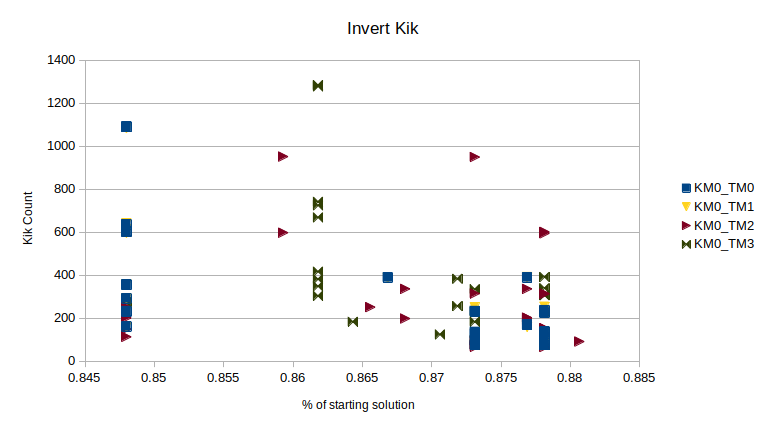
\includegraphics[scale=0.36]{InvertDist}
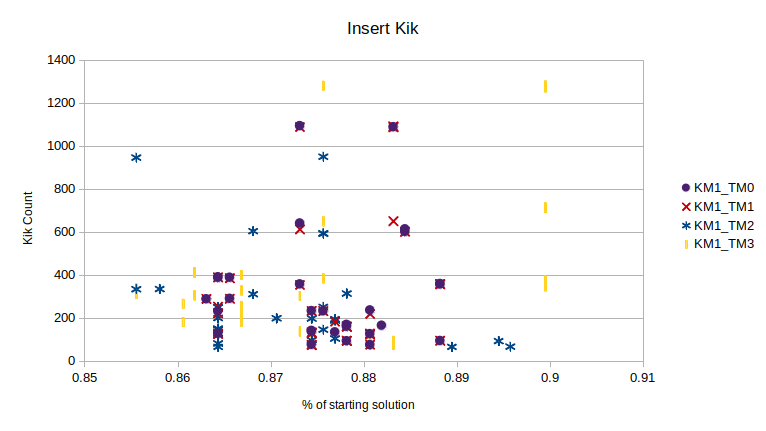
\includegraphics[scale=0.36]{InsertDist}
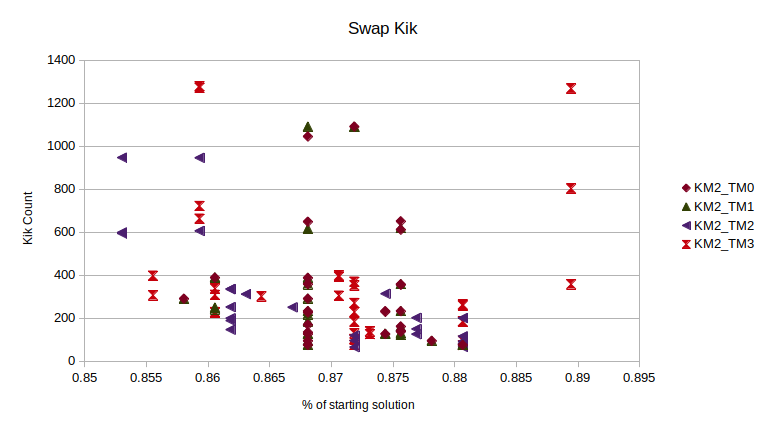
\includegraphics[scale=0.36]{SwapDist}
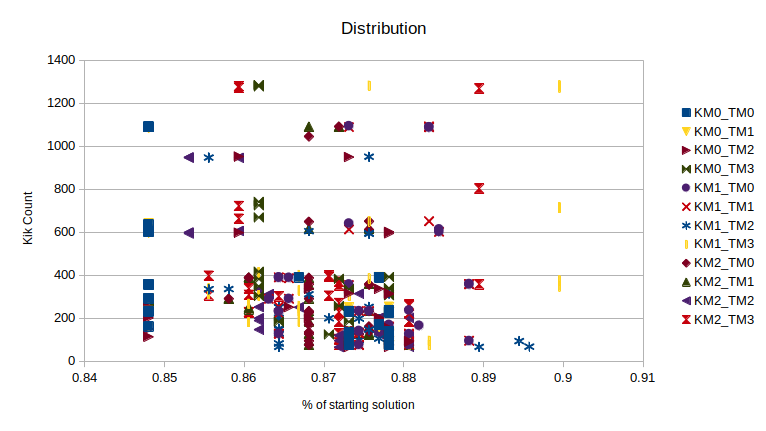
\includegraphics[scale=0.36]{OverallDist}

Jak można (albo i nie) zauważyć, różne tryby kików zupełnie inaczej wpływają na ich efektywność - najlepiej to widać dal Inverta, dla którego albo mała ich liczba jest 'bardzo trafiona', albo względnie słaba, ale jest mało wartości pośrednich, natomiast dla posostałych 2 trybów jest zupełnie na odwrót, przy czym widać, że Insert osiąga nieco lepsze pod względem dystrybucji (większa koncentracja ze strony 'lewej') wyniki od swapa (który jednak bardziej koncentruje się w 'środku')

\newpage
Przejdźmy teraz do Tabeli 2, w której to zawrzemy wyniki analogiczne do tych z Tabeli 1.

\begin{table}[h!]
	\centering
	\begin{tabular}{c|c|c||c|c|c|c}
	Tabela 2.\\
KikMode & TabuSizeMode & EnhanceMode & Min & Average & Max & StDev \\
\hline
Invert & 7 & Tabu * 2 + 1 & \textbf{\textit{2663}} & 2673.(3) & 2685 & 9.89275829415974 \\
 &  & Rest & 2672 & 2680 & 2685 & 6.26099033699945 \\
\cline{2-7}
 & Size / 10 & Tabu * 2 + 1 & \textbf{\textit{2659}} & 2673.(3) & 2679 & 7.81451640644948 \\
 &  & Rest & 2672 & 2676.(6) & 2679 & 3.61478445646025 \\
\cline{2-7}
 & $\sqrt(Size)$ & Tabu * 2 + 1 & \textbf{2657} & 2669.(3) & 2679 & 10.0531918646103 \\
 &  & Rest & 2672 & 2676.(6) & 2679 & 3.61478445646025 \\
\cline{2-7}
 & $log_2(Size)$ & Tabu * 2 + 1 &  \textbf{\textit{2672}} & 2679.(3) & 2685 & 6.47044563122727 \\
 &  & Rest &  \textbf{\textit{2672}} & 2680 & 2685 & 6.26099033699945 \\
\hline
Insert & 7 & Tabu * 2 + 1 & 2685 & 2685 & 2685 & 0 \\
 &  & Rest &  \textbf{\textit{2682}} & 2684 & 2685 & 1.54919333848294 \\
\cline{2-7}
 & Size / 10 & Any &  \textbf{\textit{2679}} & 2679 & 2679 & 0 \\
\cline{2-7}
 & $\sqrt(Size)$ & Tabu * 2 + 1 &  \textbf{\textit{2670}} & 2676 & 2679 & 4.64758001544889 \\
 &  & Rest & 2679 & 2679 & 2679 & 0 \\
\cline{2-7}
 & $log_2(Size)$ & Tabu * 2 + 1 & 2685 & 2685 & 2685 & 0 \\
 &  & Rest &  \textbf{\textit{2682}} & 2684 & 2685 & 1.54919333848294 \\
\hline
Swap & 7 & Tabu * 2 + 1 & 2685 & 2685 & 2685 & 0 \\
 &  & Rest & 2671 & 2680.(3) & 2685 & 7.22956891292053 \\
\cline{2-7}
 & Size / 10 & Tabu * $\sqrt(Size)$ &  \textbf{\textit{2665}} & 2676.(6) & 2679 & 5.71547606649408 \\
 &  & Rest &  \textbf{\textit{2665}} & 2674.(3) & 2679 & 7.22956891292053 \\
\cline{2-7}
 & $\sqrt(Size)$ & Any &  \textbf{\textit{2665}} & 2674.(3) & 2679 & 7.22956891292053 \\
\cline{2-7}
 & $log_2(Size)$ & Any &  \textbf{\textit{2671}} & 2680.(3) & 2685 & 7.22956891292053 \\
\end{tabular}
\end{table}

Wypunktujmy kilka obserwacji na podstawie tej tabeli:
\begin{itemize}
	\item Jak można tutaj zauważyć, niektóre przypadki się nam 'zlepiły ze sobą' (Tam gdzie cała kategoria osiągała takie same wyniki zaznaczone to zostało jako 'Any', natomiast tam, gdzie jedna się wyróżniła, to została nazwana, a pozostałe zbiorczo funkcjonują pod nazwą 'Rest').
	\item Jednak zauważalne jest to że mimmo wszystko najepsz wynik został osiągnięty między innymi dzięki zastosowaniu długości listy Tabu równej $\sqrt{n}$.
	\item Pojawia się nam tutaj także ciekawa własność, że zaraz po najlepszym, wyniku - 2657 - bardzo blisko są wyniki osiągane przez Kika tryby Swap - w przeciwieństwie do przypadku poprzedniego, gdzie Swap prezentował się dobrze, ale nie wyróżniająco.
	\item Na koniec jeszcze tylko zwróćmy uwagę na to, jak mało od siebie się różnią wartości maksymalne - co oznacza, że wiele zaczyna 'asymptocznie' zbiegać do podobnego wyniku.
\end{itemize}

I na koniec w tej sekcji jeszcze mini-tabela 3, w której to jedynie pokażemy, jakie były najmniejsze, oraz największe osiągnięte wartości funkcji celu dla poszczególnych trybów otoczenia (Wszystkie wyniki osiągnęły łącznie jedynie 12 różnych wartości, dlatego uznajemy ten przypadek za 'zdegenerowany' dla naszych potrzeb i tak samo najmniej się zajmiemy jego analizą):

\begin{table}[h!]
	\centering
	\begin{tabular}{c||c|c|c}
	Tabela 3.\\
NeiMode & Min Score & Max Score \\
\hline
Invert & 276539 & 278997 \\
Insert & 301883 & 301883 \\
Swap & 302798 & 303465 \\
\end{tabular}
\end{table}

Jak widać, granice są bardzo wyraźne, oraz można stwierdzić, że bezsprzecznie otoczenie rodzaju Invert zadziałał tu najlepiej.

\newpage
\subsection{porównanie wpływu listy długoterminowej}

Dla porównania wpływu korzystania z listy długoterminowej (LTM) przetestowane zostały instancje o 'prosperujących' hiperparametrach ustalonych wcześniej (jakie dokładnie - zaraz), oraz przy czasie równym 60 sekund na każdy przebieg. W tabeli 4. zostały umieszczone wyniki uzyskane z- i bez LTM, oraz (aby być może zobaczyć różnicę w zależności od parametrów) zrobione to zostało dla 2 wariantów:
\begin{itemize}
	\item Lista tabu długości = 7
	\item Lista tabu długości = $\sqrt{n}$
\end{itemize}
Wartości stałe dla każdego przebiegu:
\begin{itemize}
	\item Rodzaj otoczenia - \textit{Invert}
	\item Rodzaj 'Kika' - \textit{Invert}
	\item Wielkość 'Kika' - 7
	\item Liczba iteracji bez poprawy - $|Tabu|*2 + 1$
\end{itemize}

\begin{table}[h!]
	\centering
	\begin{tabular}{c||c|c|c|c}
	Tabela 4.\\
n & LTM 7 & LTM Sqrt & No LTM 7 & No LTM Sqrt \\
\hline
51 & 0.887966804979253 & 0.887966804979253 & 0.887966804979253 & 0.887966804979253 \\
52 & 0.961129446277961 & 0.961129446277961 & 0.961129446277961 & 0.961129446277961 \\
70 & 0.847989949748744 & 0.858040201005025 & 0.85929648241206 & 0.858040201005025 \\
76(1) & 0.899671052631579 & 0.894736842105263 & 0.894736842105263 & 0.893092105263158 \\
76(2) & 0.834281742424821 & 0.829515509352969 & 0.829187067009876 & 0.834304657006897 \\
99 & 0.856645789839944 & 0.846903270702853 & 0.848295059151009 & 0.856645789839944 \\
100(1) & 0.866021540205685 & 0.863227791724026 & 0.866021540205685 & 0.863227791724026 \\
100(2) & 0.863545047133364 & 0.860531602534384 & 0.868567454798331 & 0.863429145418019 \\
100(3) & 0.889518174133559 & 0.889391377852916 & 0.889814032121724 & 0.89429416737109 \\
100(4) & 0.867777241268308 & 0.869628198937711 & 0.86934653146628 & 0.866288427490745 \\
100(5) & 0.903881849729642 & 0.906827536114922 & 0.898232588168832 & 0.901904608183359 \\
101 & 0.865951742627346 & 0.857908847184987 & 0.859249329758713 & 0.867292225201072 \\
105 & 0.854738706820195 & 0.854738706820195 & 0.854738706820195 & 0.854738706820195 \\
107 & 0.957647814910026 & 0.953770351328192 & 0.956319622964867 & 0.954755784061697 \\
124 & 0.900335545447767 & 0.900335545447767 & 0.900335545447767 & 0.900335545447767 \\
127 & 0.903279508484319 & 0.892126342821736 & 0.900218733436354 & 0.902428463714885 \\
130 & 0.901809510450274 & 0.899424884275494 & 0.915556178987235 & 0.882311684668256 \\
136 & 0.86353914781804 & 0.870348223093241 & 0.85543809415729 & 0.861278185643327 \\
144 & 0.963224197887278 & 0.963224197887278 & 0.962682894823174 & 0.962682894823174 \\
150(1) & 0.934064389146633 & 0.934064389146633 & 0.934064389146633 & 0.934064389146633 \\
150(2) & 0.885638044410559 & 0.870612154134502 & 0.865942374281267 & 0.879411671272912 \\
150(3) & 0.847647970643131 & 0.846920375818544 & 0.844642687672013 & 0.848723545601215 \\
152 & 0.946244532703233 & 0.943994771504701 & 0.947451108541551 & 0.941267407370167 \\
195 & 0.916156202143951 & 0.916156202143951 & 0.916156202143951 & 0.916156202143951 \\
200(1) & 0.87395420200909 & 0.87395420200909 & 0.87395420200909 & 0.87395420200909 \\
200(2) & 0.869422701969538 & 0.867077340416514 & 0.857441577891435 & 0.858939218401198 \\
225(1) & 0.907264780832254 & 0.913685349429836 & 0.907264780832254 & 0.913685349429836 \\
225(2) & 0.886194844910441 & 0.887287024901704 & 0.887505460899956 & 0.884010484927916 \\
226 & 0.886301754689256 & 0.886215316794883 & 0.885858760480595 & 0.885858760480595 \\
264 & 0.909911728542328 & 0.910168651703951 & 0.922133930373823 & 0.922133930373823 \\
280 & 0.888403361344538 & 0.88436974789916 & 0.889747899159664 & 0.893109243697479 \\
299 & 0.860103982566619 & 0.860103982566619 & 0.860103982566619 & 0.860103982566619 \\
318(1) & 0.887664884860064 & 0.887664884860064 & 0.883132456657385 & 0.885124286091746 \\
318(2) & 0.887664884860064 & 0.887664884860064 & 0.883132456657385 & 0.885124286091746 \\
439 & 0.885270769472609 & 0.891880845712489 & 0.859081977521025 & 0.891880845712489 \\
575 & 0.888527461528838 & 0.890404103590642 & 0.889153008882772 & 0.890404103590642 \\
783 & 0.883111954459203 & 0.883111954459203 & 0.883111954459203 & 0.883111954459203 \\
1002 & 0.88141324961354 & 0.88141324961354 & 0.88141324961354 & 0.88141324961354 \\

\end{tabular}
\end{table}

Na danej tabeli zostało wykonane kilka testów Wilcoxona (przy użyciu pythonowej biblioteki \textbf{\textit{scipy.stats}}, aby móc w miarę rzetelny sposób zbadać dane zjawisko. Wyniki danych testów przedstawione zostały w Tabeli 5, wraz z przyjętymi oznaczeniami z Tabeli 4. oraz z dodatkowymi (przy trybie - Mode):
\begin{itemize}
	\item L. (\textit{less}) - Hipoteza, że Lewa strona wyrażenia jest 'Lepsza' od Prawej
	\item 2. - (\textit{two-sided}) - Hipoteza, że obie strony są od siebie niezależne
	\item P. (\textit{pratt}) - uwzględnienie zer przy wyliczeniu rang, ale pominięcie ich przy końcowej statystyce
	\item W. (\textit{wilcox}) - odrzucenie różnic zerowych
	\item Z. (\textit{zsplit}) - uwzględnienie zer przy wyliczaniu rang, oraz równomierna dystrybucja przy wyliczaniu końcowej statystyki.
\end{itemize}

Przejdźmy do tabelki:
\begin{table}[h!]
	\centering
	\begin{tabular}{c||c|c|c|c|c|c|c|c}
	Tabela 5.\\
\multirow {2}{*}{Mode} & \multicolumn{2}{c|}{LTM-7 : LTM-Sqrt} & \multicolumn{2}{c|}{NoLTM-7 : NoLTM-Sqrt} & \multicolumn{2}{c|}{LTM-7 : NoLTM-7} & \multicolumn{2}{c}{LTM-Sqrt : NoLTM-Sqrt} \\
\cline{2-9}
 & Stat & P-Val & Stat & P-Val & Stat & P-Val & Stat & P-Val \\
 \hline
L.P. & 420 & 0.920489778898223 & 220 & 0.059777402992287 & 427 & 0.920623436703554 & 299 & 0.43152360785135 \\
L.W. & 212 & 0.90855218158477 & 103 & 0.054684728027371 & 235 & 0.93463641598738 & 119 & 0.281659901157887 \\
L.Z. & 465.5 & 0.916875235701623 & 265.5 & 0.062996261780571 & 466 & 0.917769251905686 & 359 & 0.43328385710822 \\
\hline
2.P. & 230 & 0.159020442203553 & 220 & 0.119554805984574 & 236 & 0.158753126592892 & 299 & 0.8630472157027 \\
2.W. & 113 & 0.182895636830461 & 103 & 0.109369456054742 & 116 & 0.13072716802524 & 119 & 0.563319802315774 \\
2.Z. & 275.5 & 0.166249528596755 & 265.5 & 0.125992523561142 & 275 & 0.164461496188629 & 359 & 0.866567714216441 \\

\end{tabular}
\end{table}

Analiza tabeli :
\begin{itemize}
	\item Najpierw zauważmy, że w większości przypadków sposoby wliczania zerowych różnic niewiele zmieniły, poza przyppadkiem ostatnim, dlatego w kolejnych podpunktach nie będziemy o tym wspominali, a ostatni przykład omówimy (niespodziewane!) na końcu 
	\item Spójrzmy teraz na porównanie ze sobą tych wariantów, gdzie w obu przypadkach była użyta LTM, albo nie. Przy Hipotezie, że jeden z tych wariantów jest 'lepszy', przy użyciu LTM można z około 91\% pewnością stwierdzić, że Lista tabu długości 7 daje lepsze wyniki niż $\sqrt{n}$. Jednakże, jeżeli nie będziemy z niej korzystać, to z około 96\% pewnością można powiedzieć, że jest całkowicie na odwrót! Jednak samo zjawisko, że jedne parametry lepiej działają w porównaniu z innymi jest samo w sobie wpisane w definicję algorytmu \textit{Tabu Search}
	\item Przy porównywaniu ze sobą opcji z- i bez użycia LTM dla długości Tabu = 7 (W dalszym ciągu przy hipotezie o 'byciu llepszym') można zauważyć, że rzeczywiście jest to na korzyść użytku
	\item W kontekście bycia 'jednakowo skutecznym' dla omawianych powyżej statystyk widać, że nie otrzymujemy zbyt wysokich wyników - są one rzędu 10-20 \%, czego można by się spodziewać, ponieważ z powyższego stwierdziliśmy, że można znacząco stwierdzić, co 'zazwyczaj' działa lepiej
	\item Zastanówmy się jeszcze nad ostatnią kolumną, czyli porównania użycia LTM dla wariantu z długością listy Tabu = $\sqrt{n}$. Przy hipotezie, że użycie LTM porawia wynik, nie otrzymujemy zbyt dobrych wyników, jednakże dla założenia, że są one sobie podobne, wartość statystyki sięga nawet 86\% pewności, że rzeczywiście są sobie jednakowe. Jednak, jest tak dla statystyk uwzględniających zerowe różnice. Kiedy je wykluczymy (Tryb W.), to wtedy nasza pewność spada aż do 56\%.\\\\
	Można by tutaj wysnuć wniosek, że w tym przypadku względnie często użycie LTM całkowicie nie wpływało na rozwiązanie (zerowe różnice), a kiedy już jakoś wpływało, to niestety rzadko kiedy coś popprawiało (ze statystyki wyżej - również dla trybu W. - widać, że z tylko 28\% pewnością stwierdzamy poprawę, czyli na 72\% lepiej jej nie używać)
\end{itemize}

Podsumowując, nie można powiedzieć, że LTM zawsze pomaga, jednakże dzieje się to na tyle często, że warto (w naszej subiektywnej ocenie) ją stosować. Dodatkowo mamy tutaj idealny przykład jak jeden parametr może diametralnie zmienić ostatecznie otrzymywane wartości.

\newpage
\subsection{Porównanie wariantów dla optymalnych parametrów}

Po przetestowaniu optymalnych parametrów przeprowadzono testy dla ustalonych instancji TSPLIB. Wykresy podzielono na dwie grupy, po lewej operacja \texttt{kick} była losowa w zadanym przedziale, po prawej deterministyczna.
\\

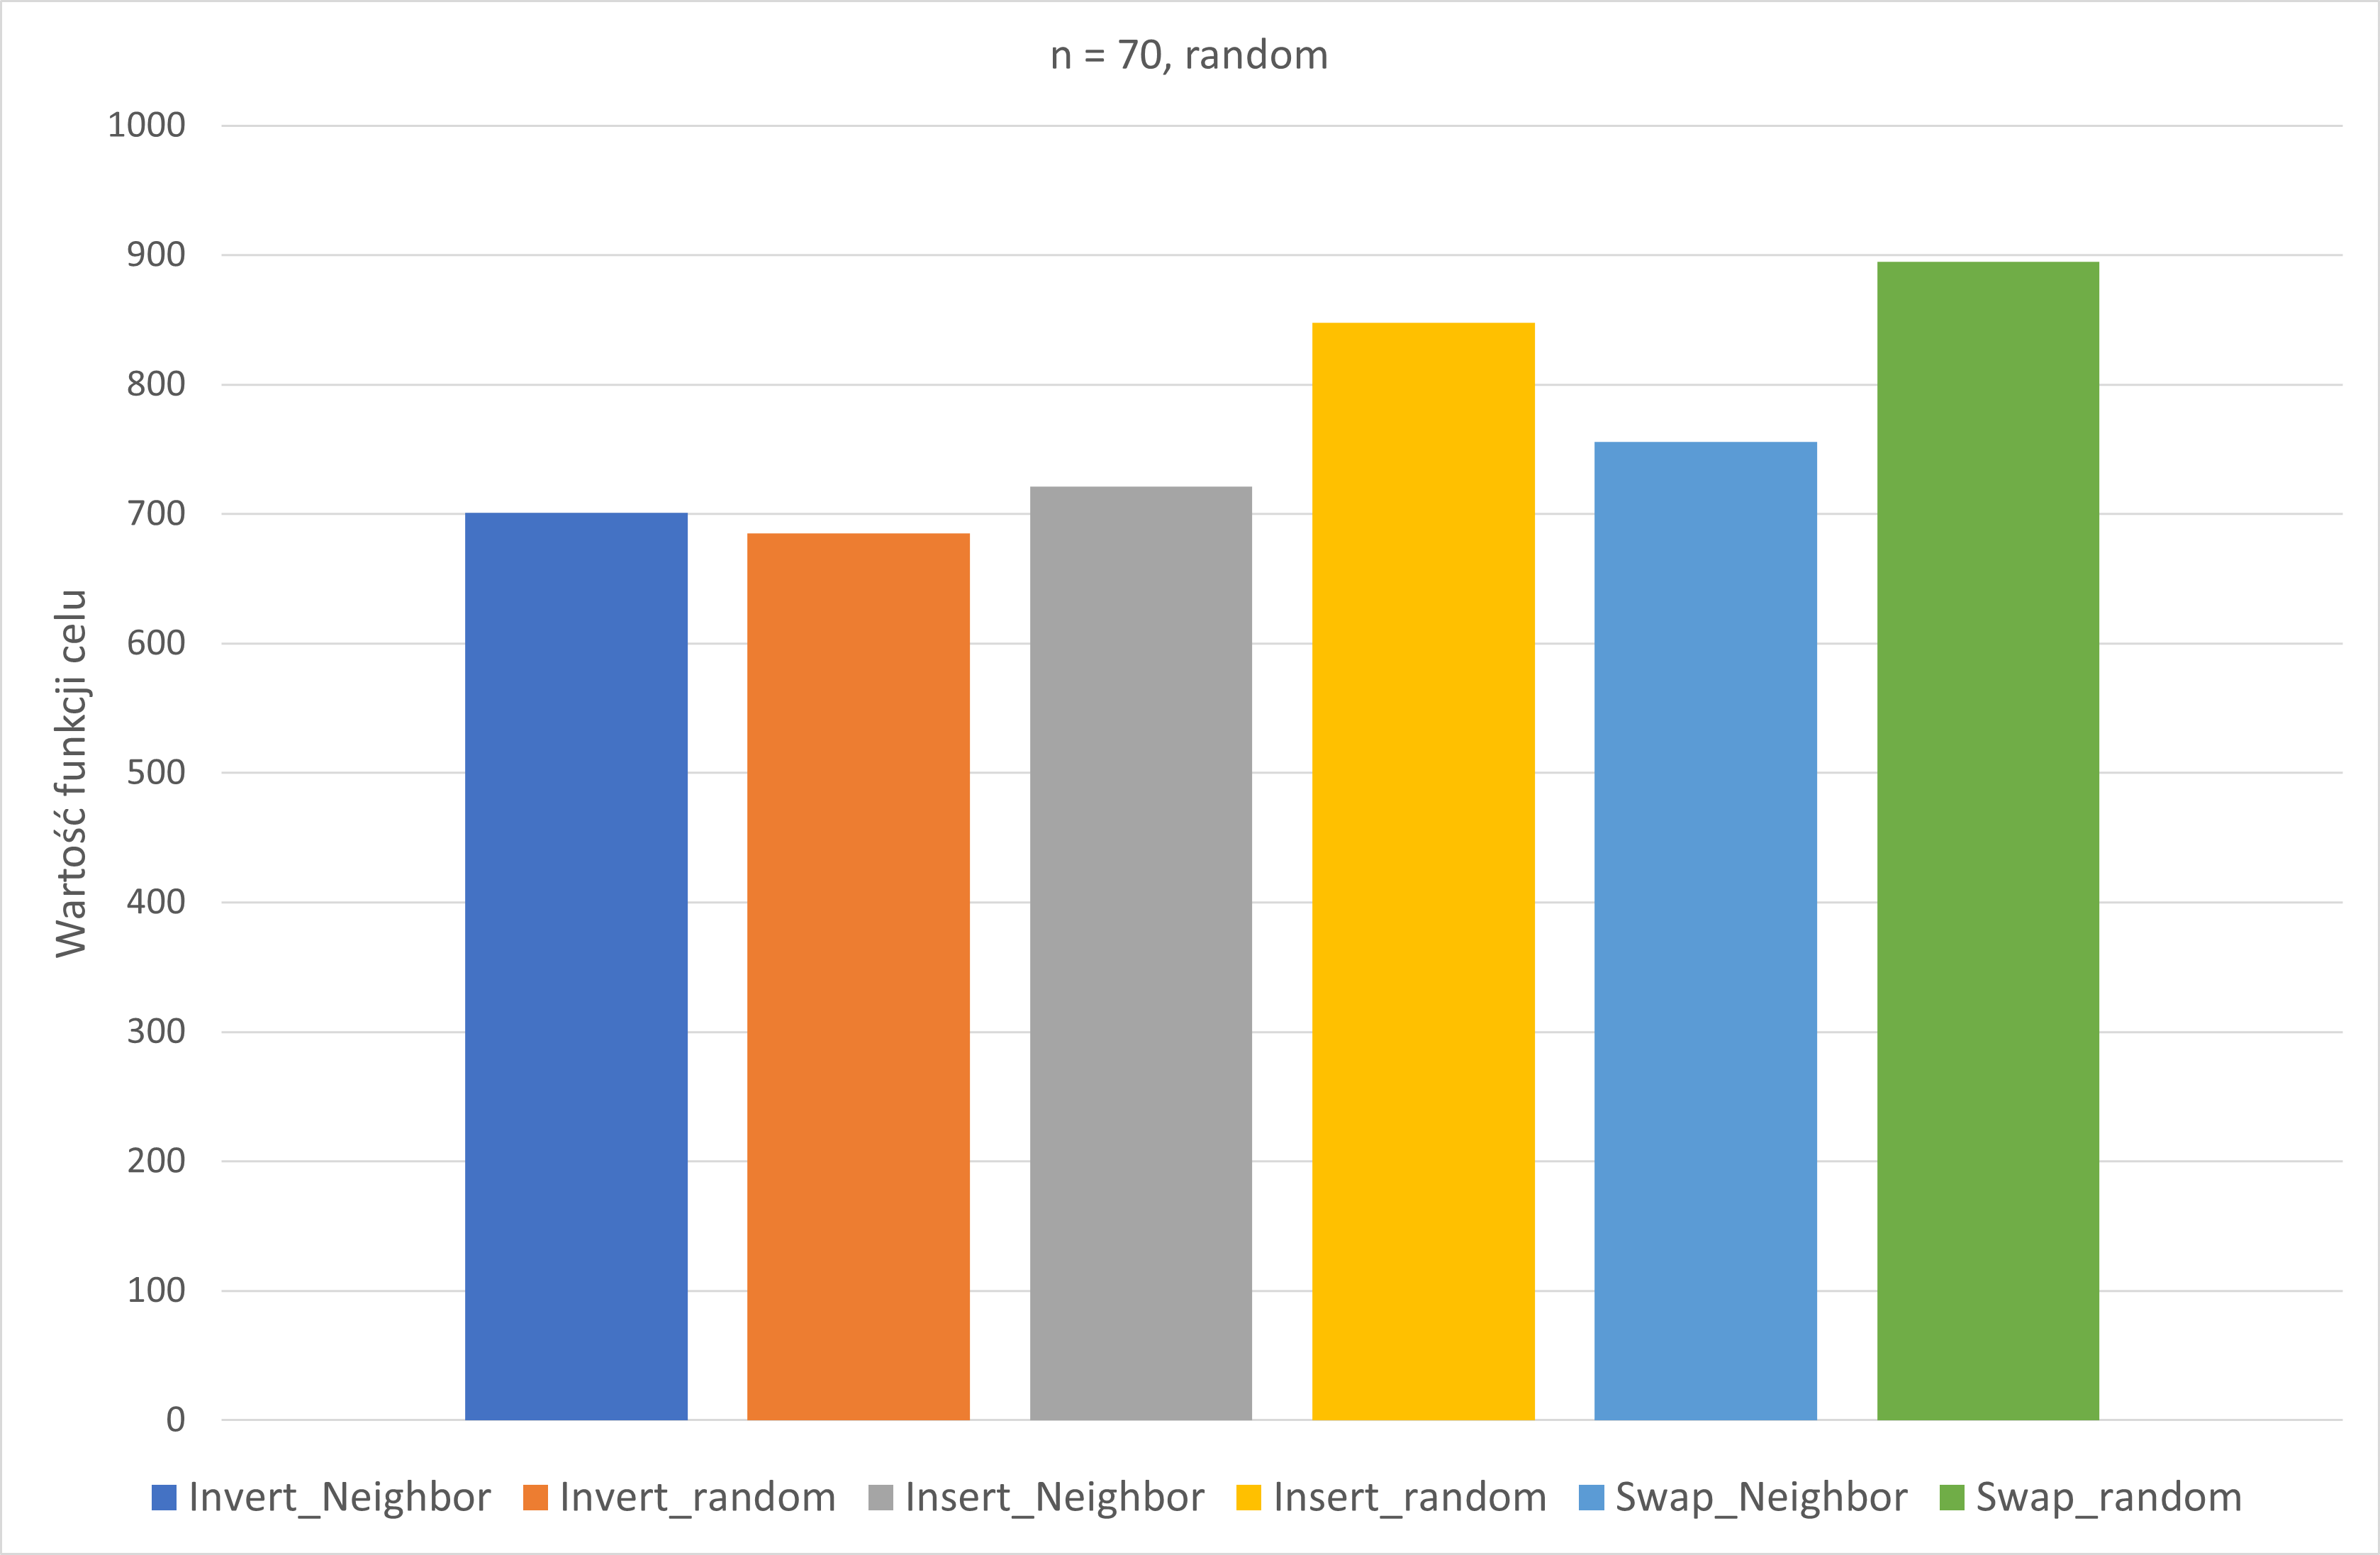
\includegraphics[scale=0.36]{70_rand}
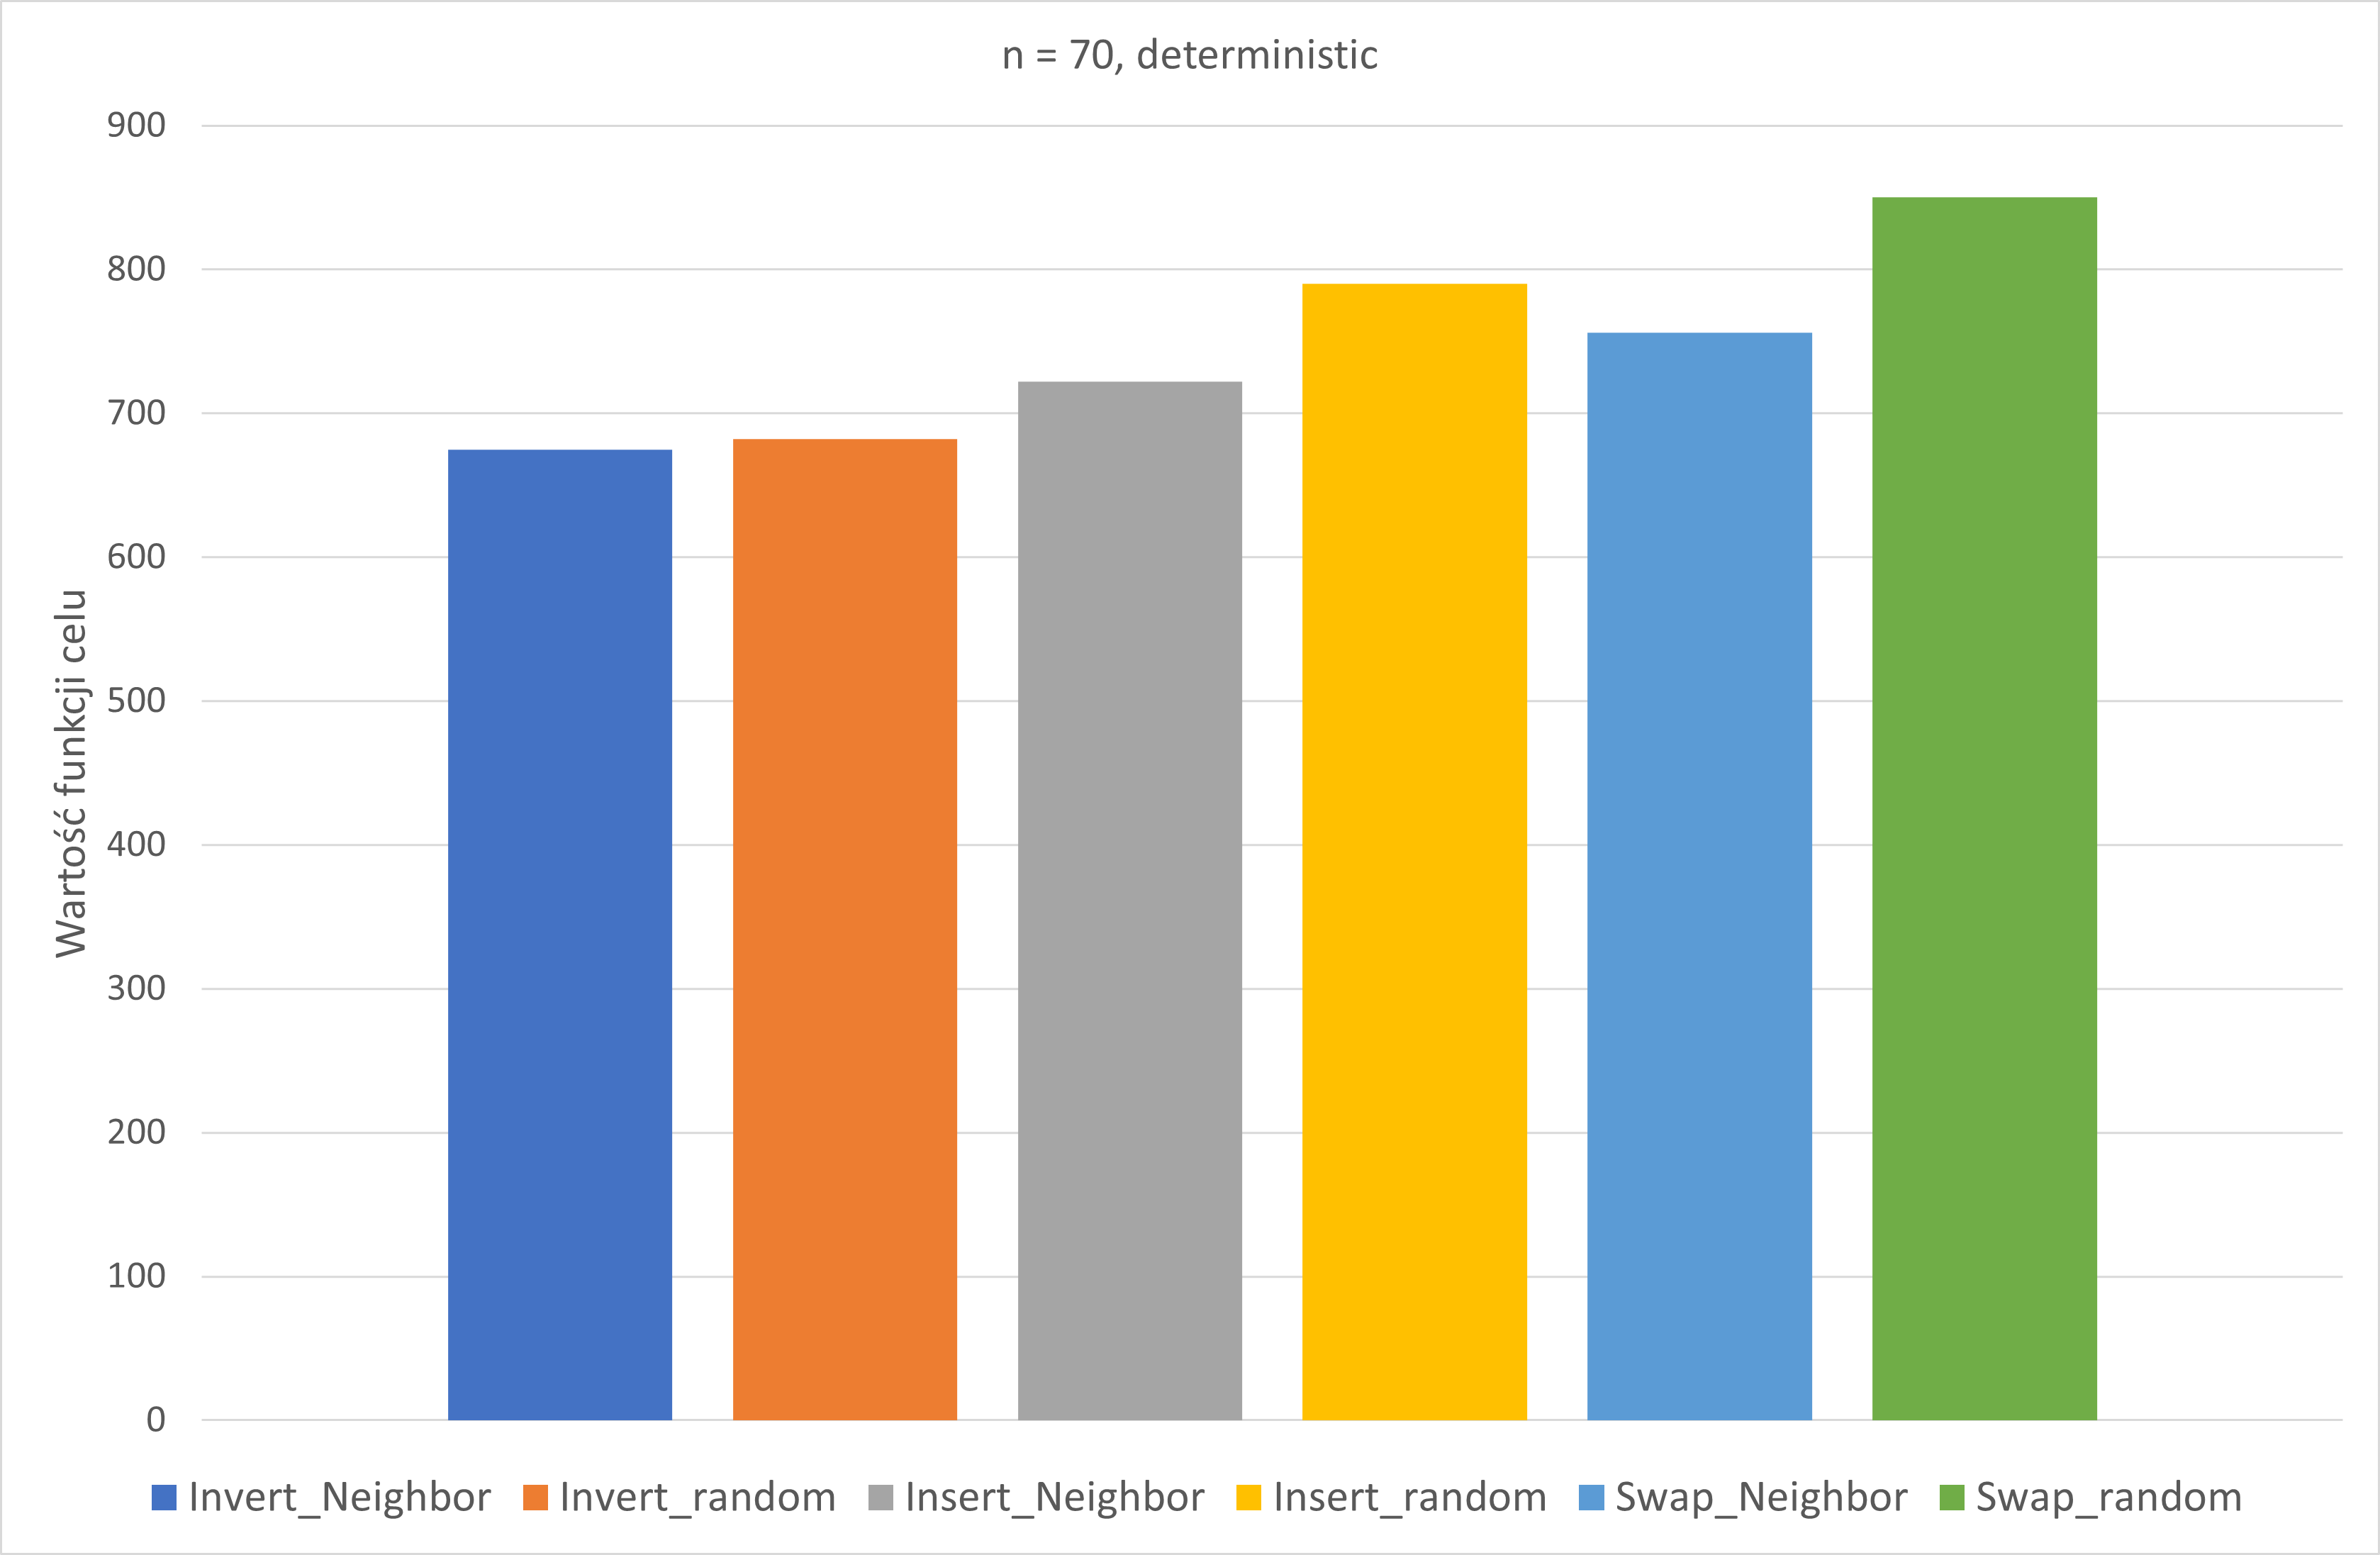
\includegraphics[scale=0.36]{70_deter}
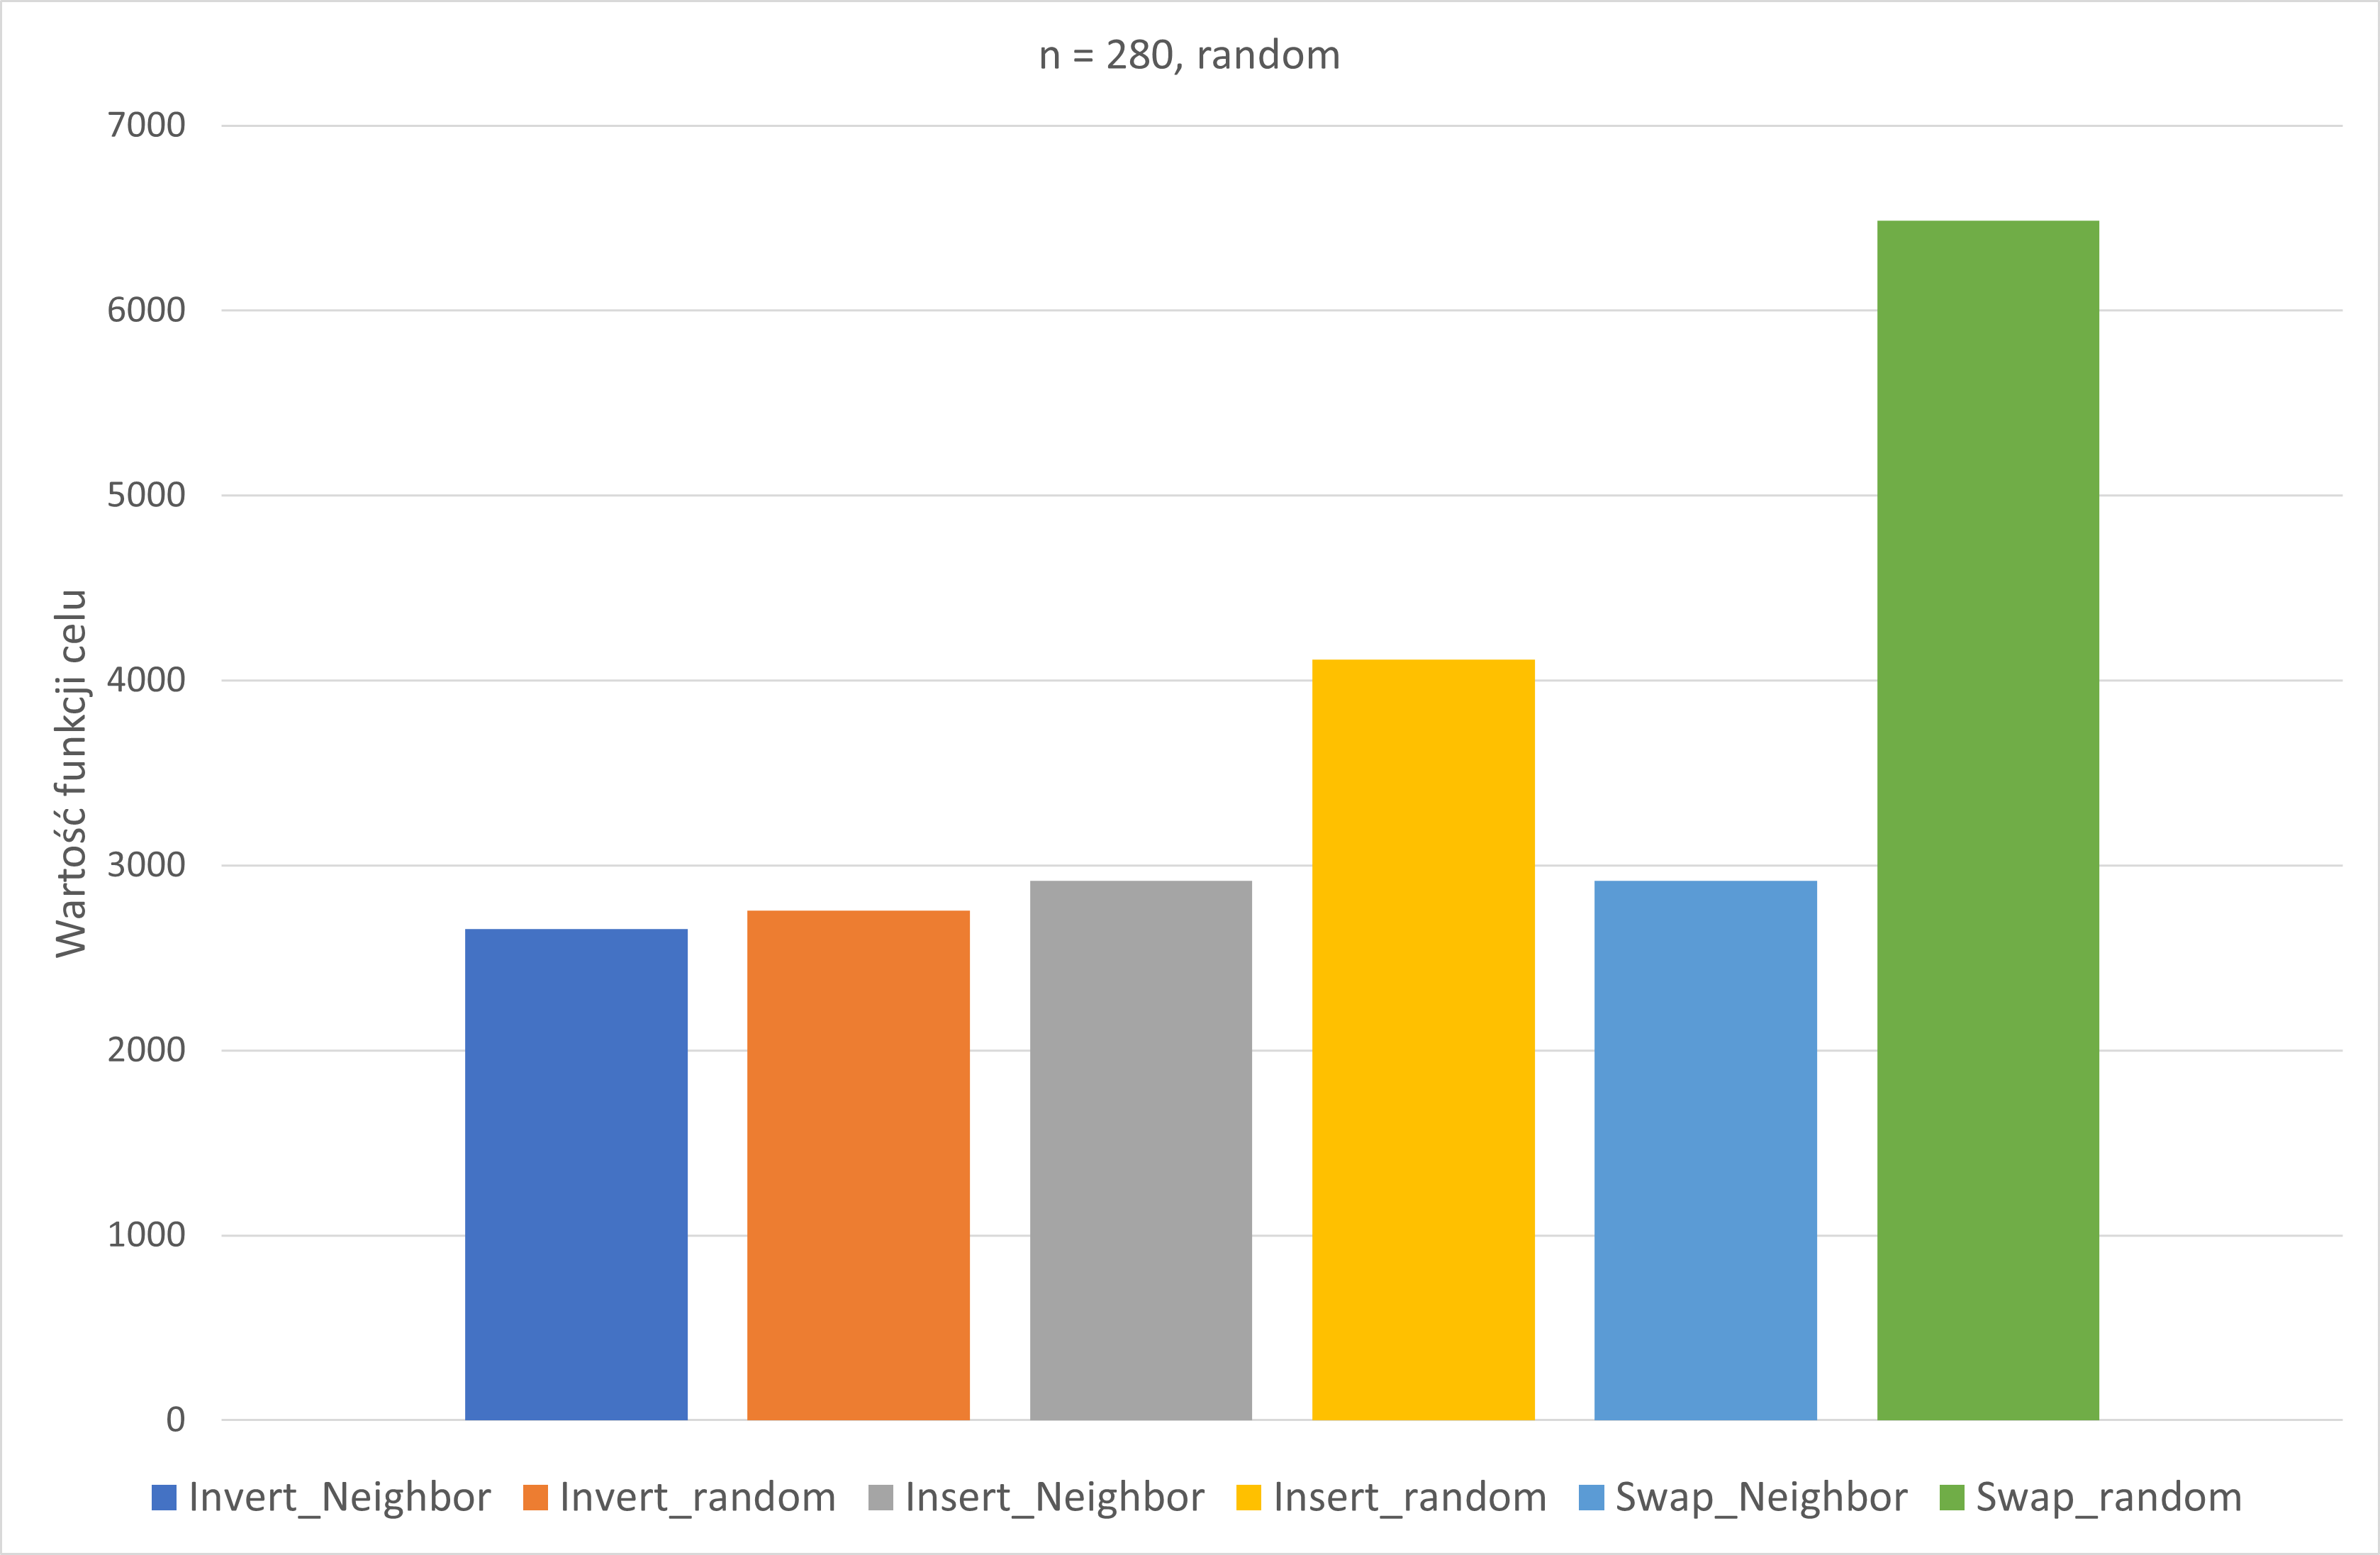
\includegraphics[scale=0.36]{280_rand}
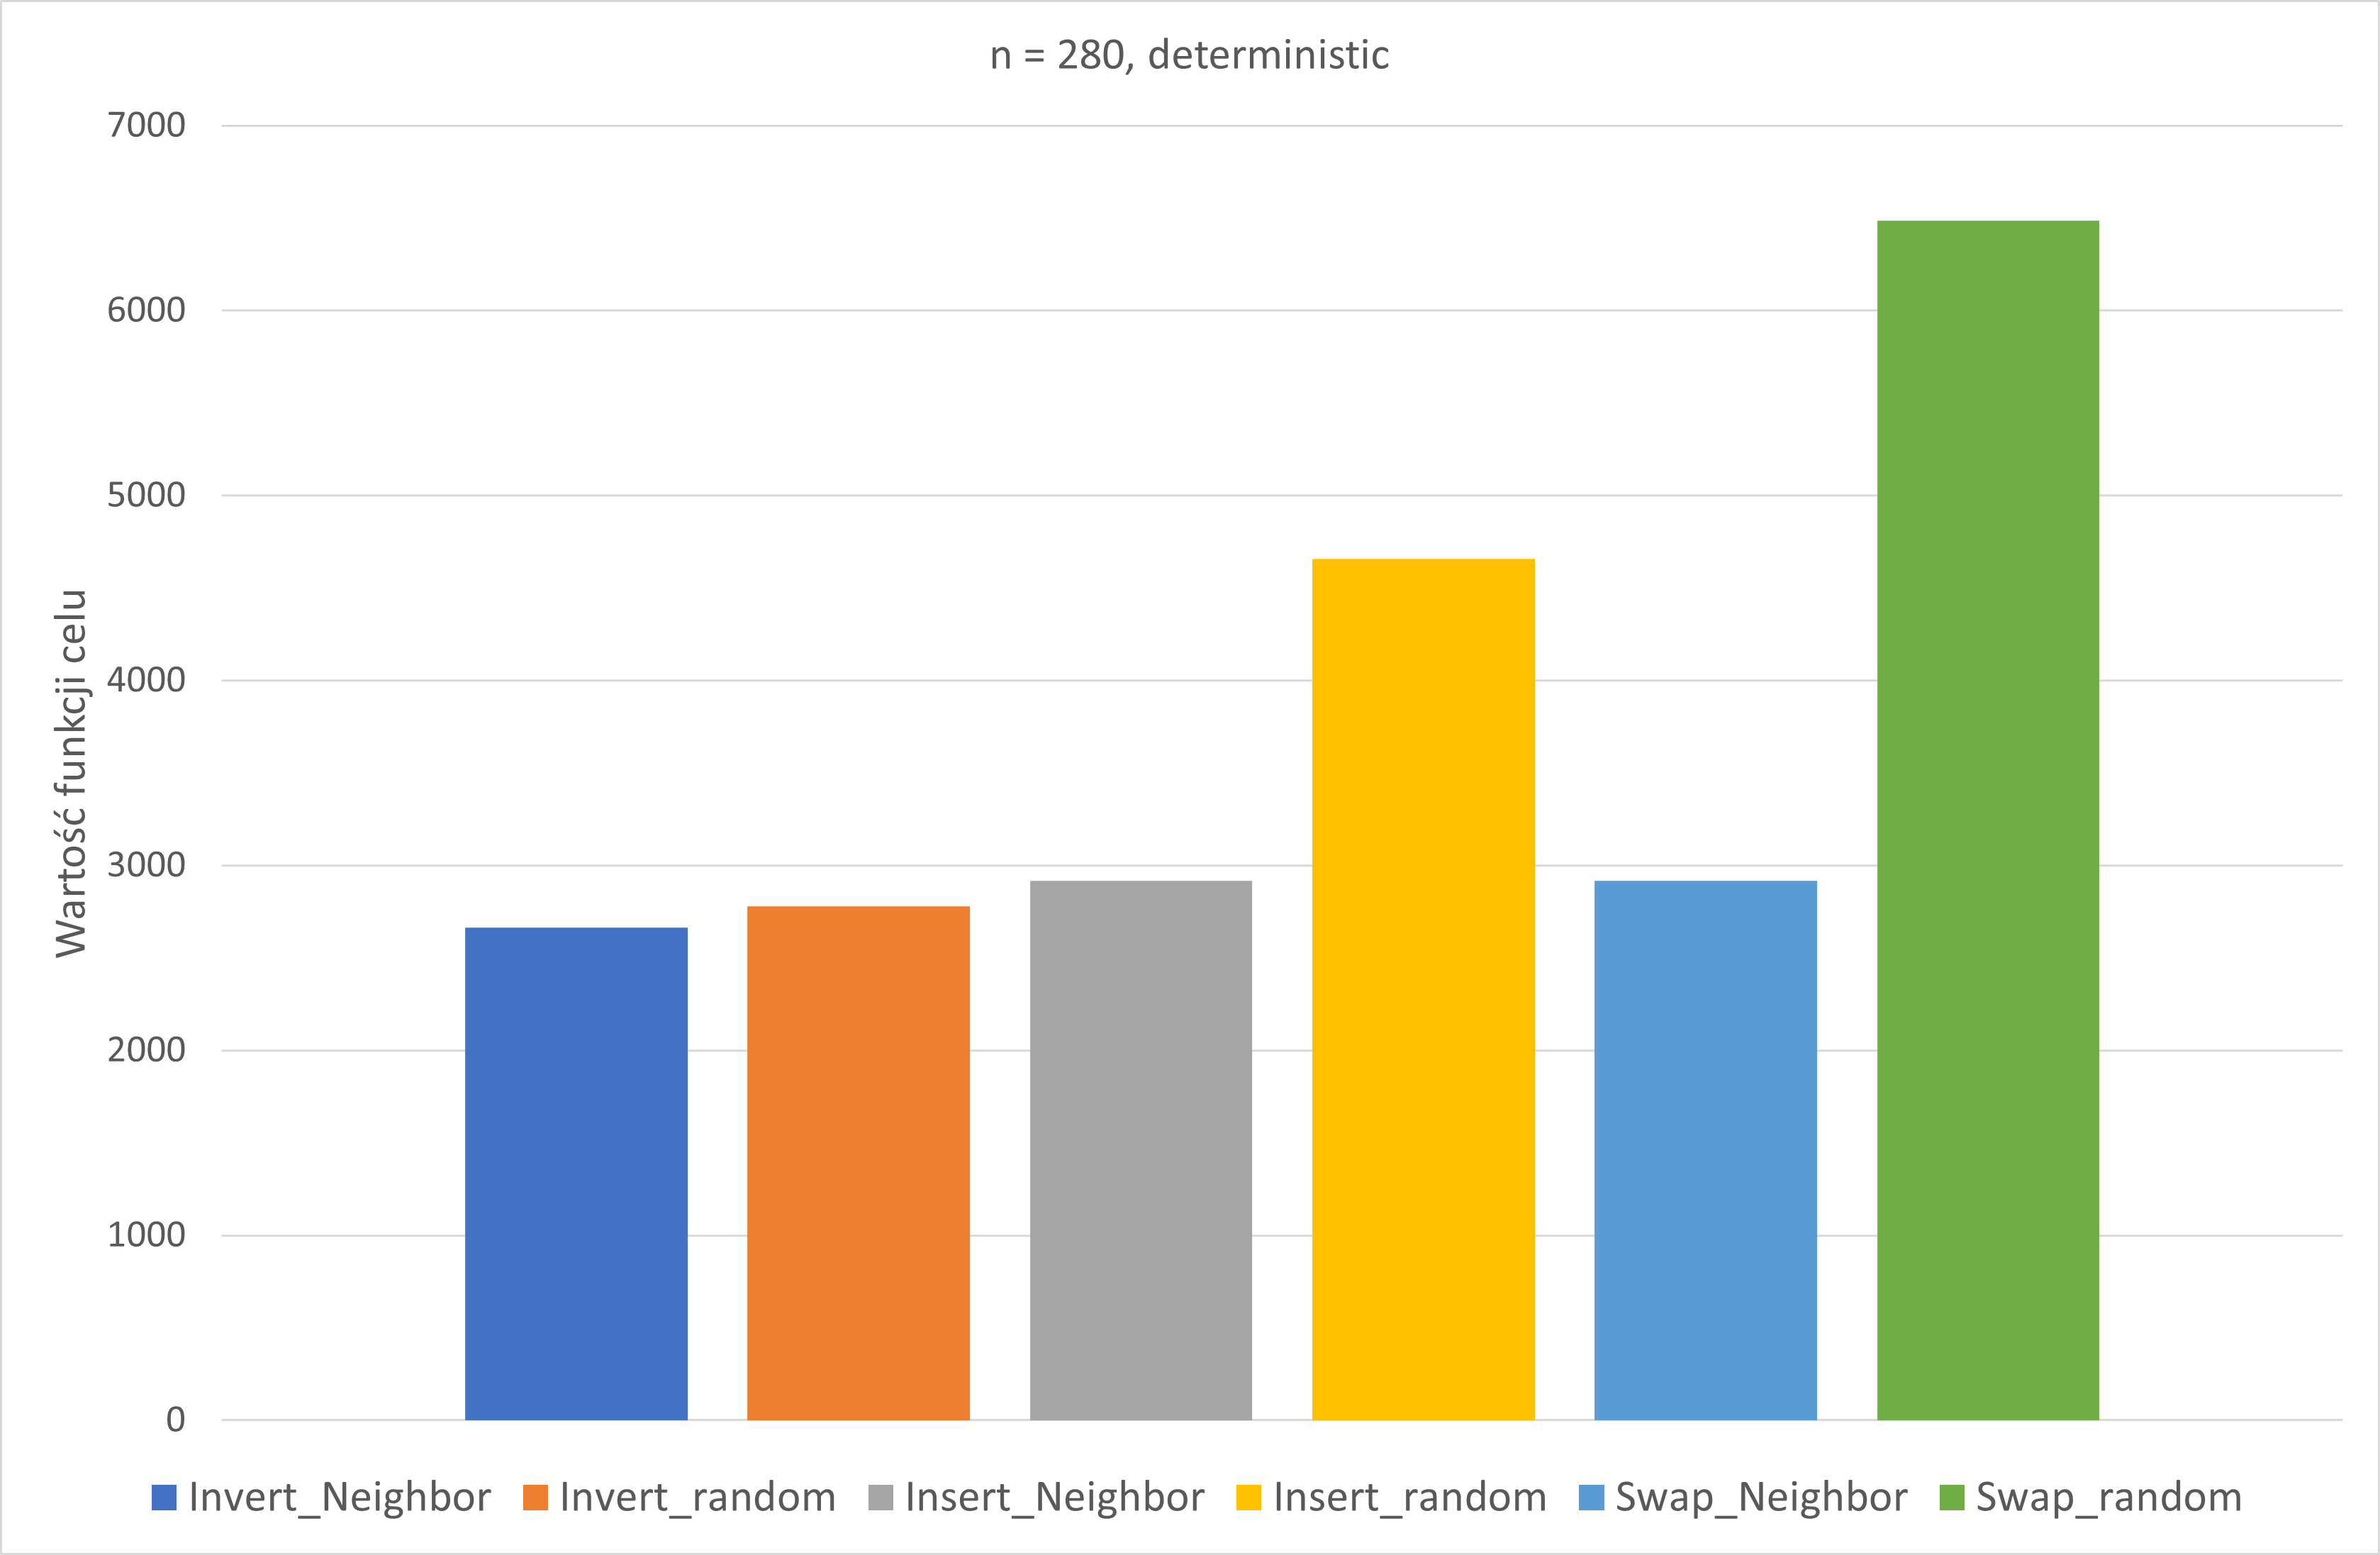
\includegraphics[scale=0.36]{280_deter}
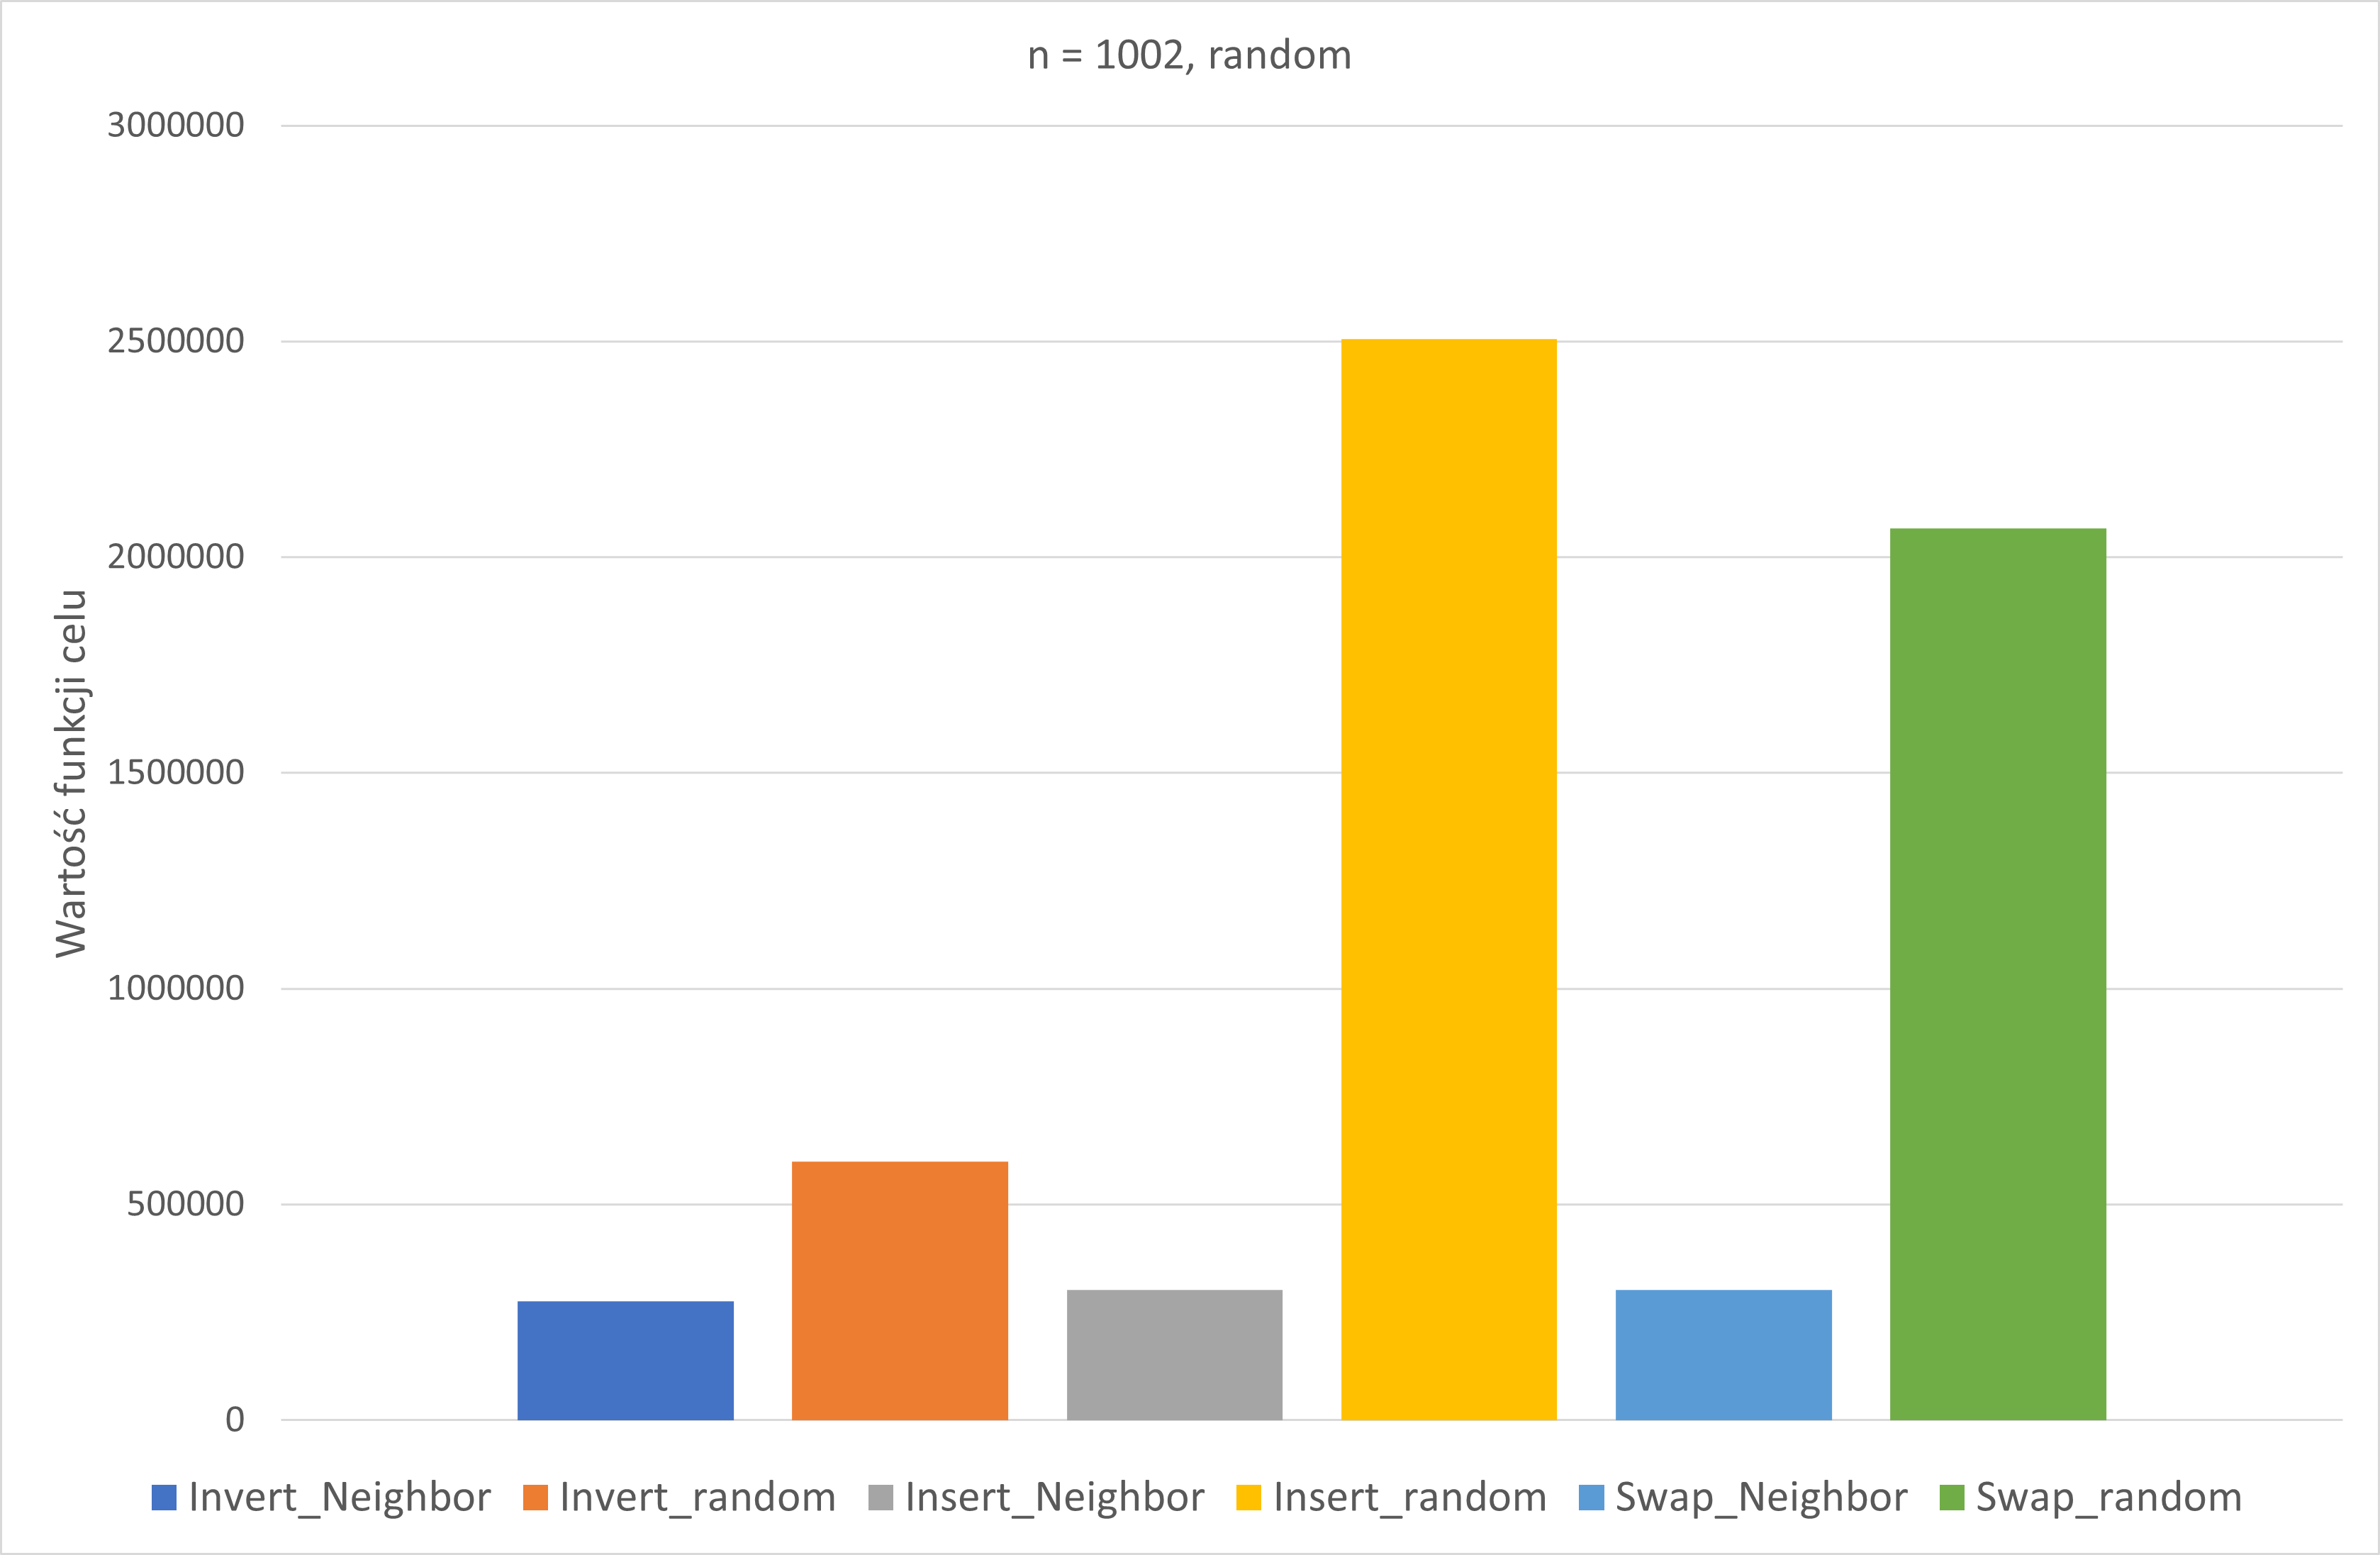
\includegraphics[scale=0.36]{1002_rand}
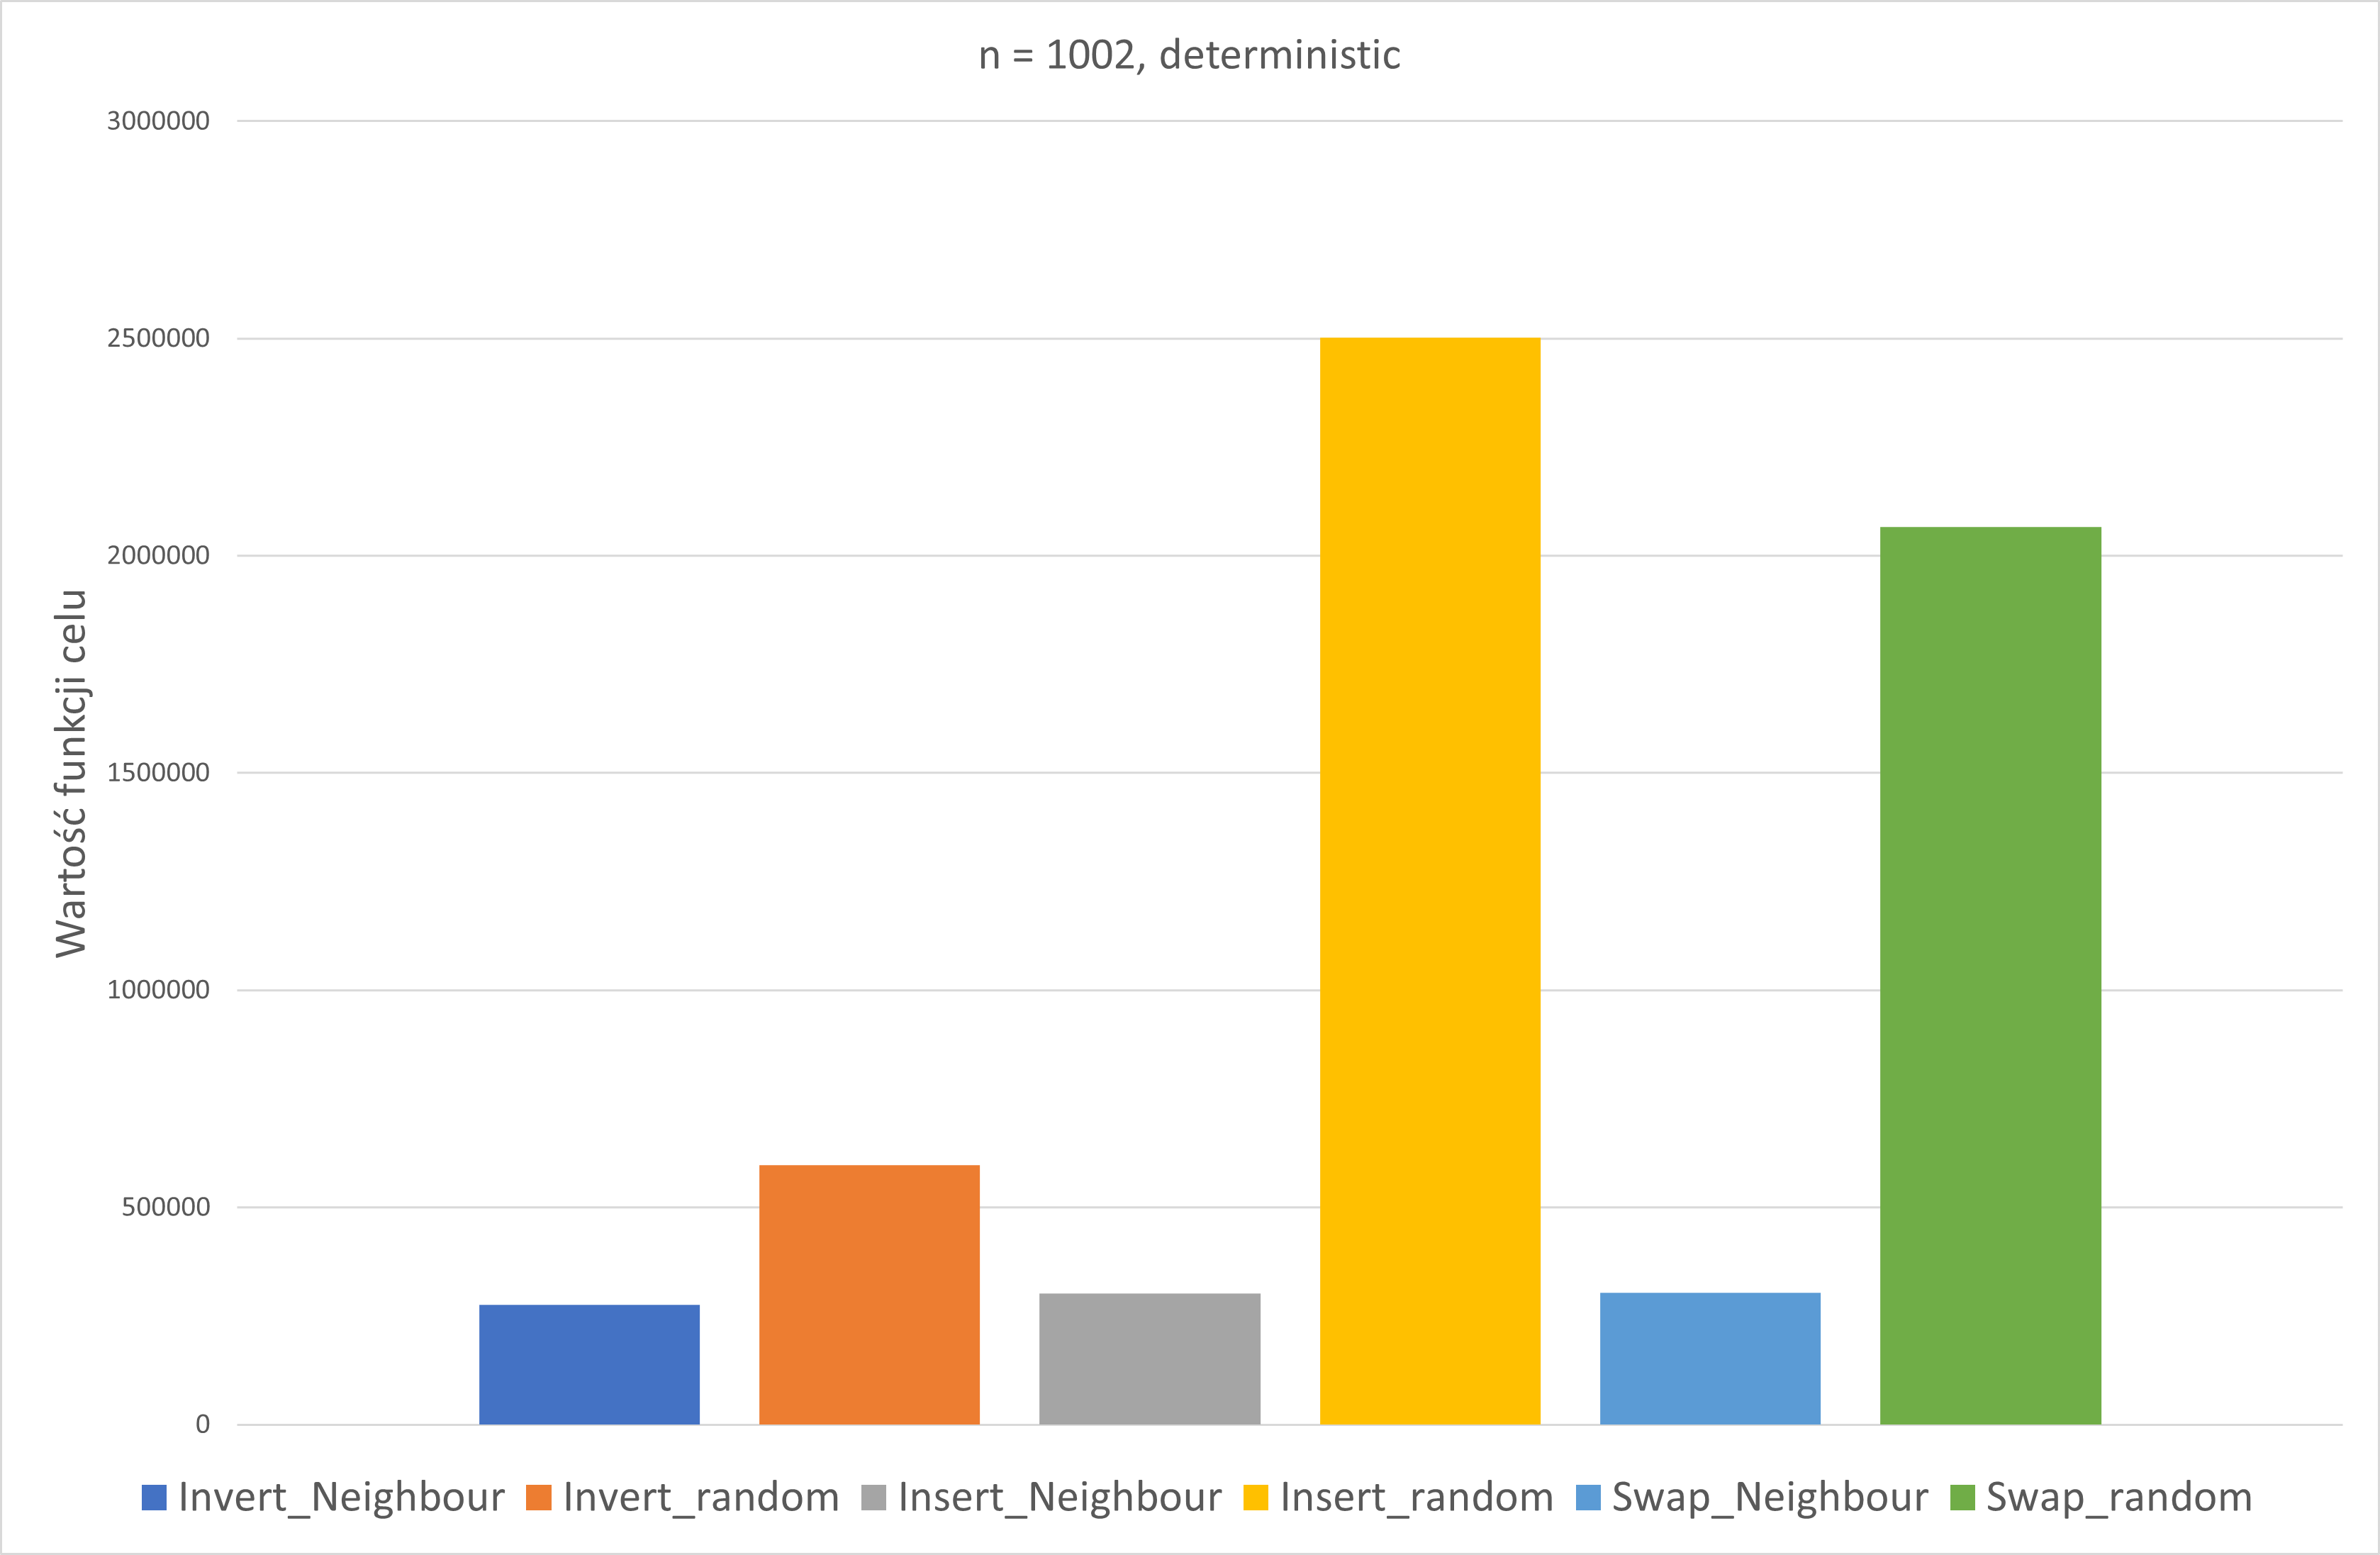
\includegraphics[scale=0.36]{1002_deter}

W obydwu wariantach operacji \texttt{kick} można zauważyć zbliżone wyniki przy wszystkich wielkościach problemu. Co więcej, wraz ze zwiększaniem się problemu bardziej klarownie widać różnice między wersjami. 
\begin{itemize}
	\item Początkowa trasa na podstawie Nearest Neighbour daje lepsze wyniki niż k-random
	\item Wszystkie otoczenia są porównywalne, najlepszy Invert, następnie Insert, najgorszy Swap
\end{itemize}

\newpage
\subsubsection{Algorytmy uwspółbieżnione}

Uwspółbieżnienie zaimplementowano na zasadzie równoległego uruchamiania kilku instancji algorytmu \texttt{TABU-Search} jednocześnie. Z oczywistych względów nie testowano zachowania deterministycznej wersji algorytmu. Niestety, ta metoda uwspółbieżnienia nie dała dobrych rezultatów:

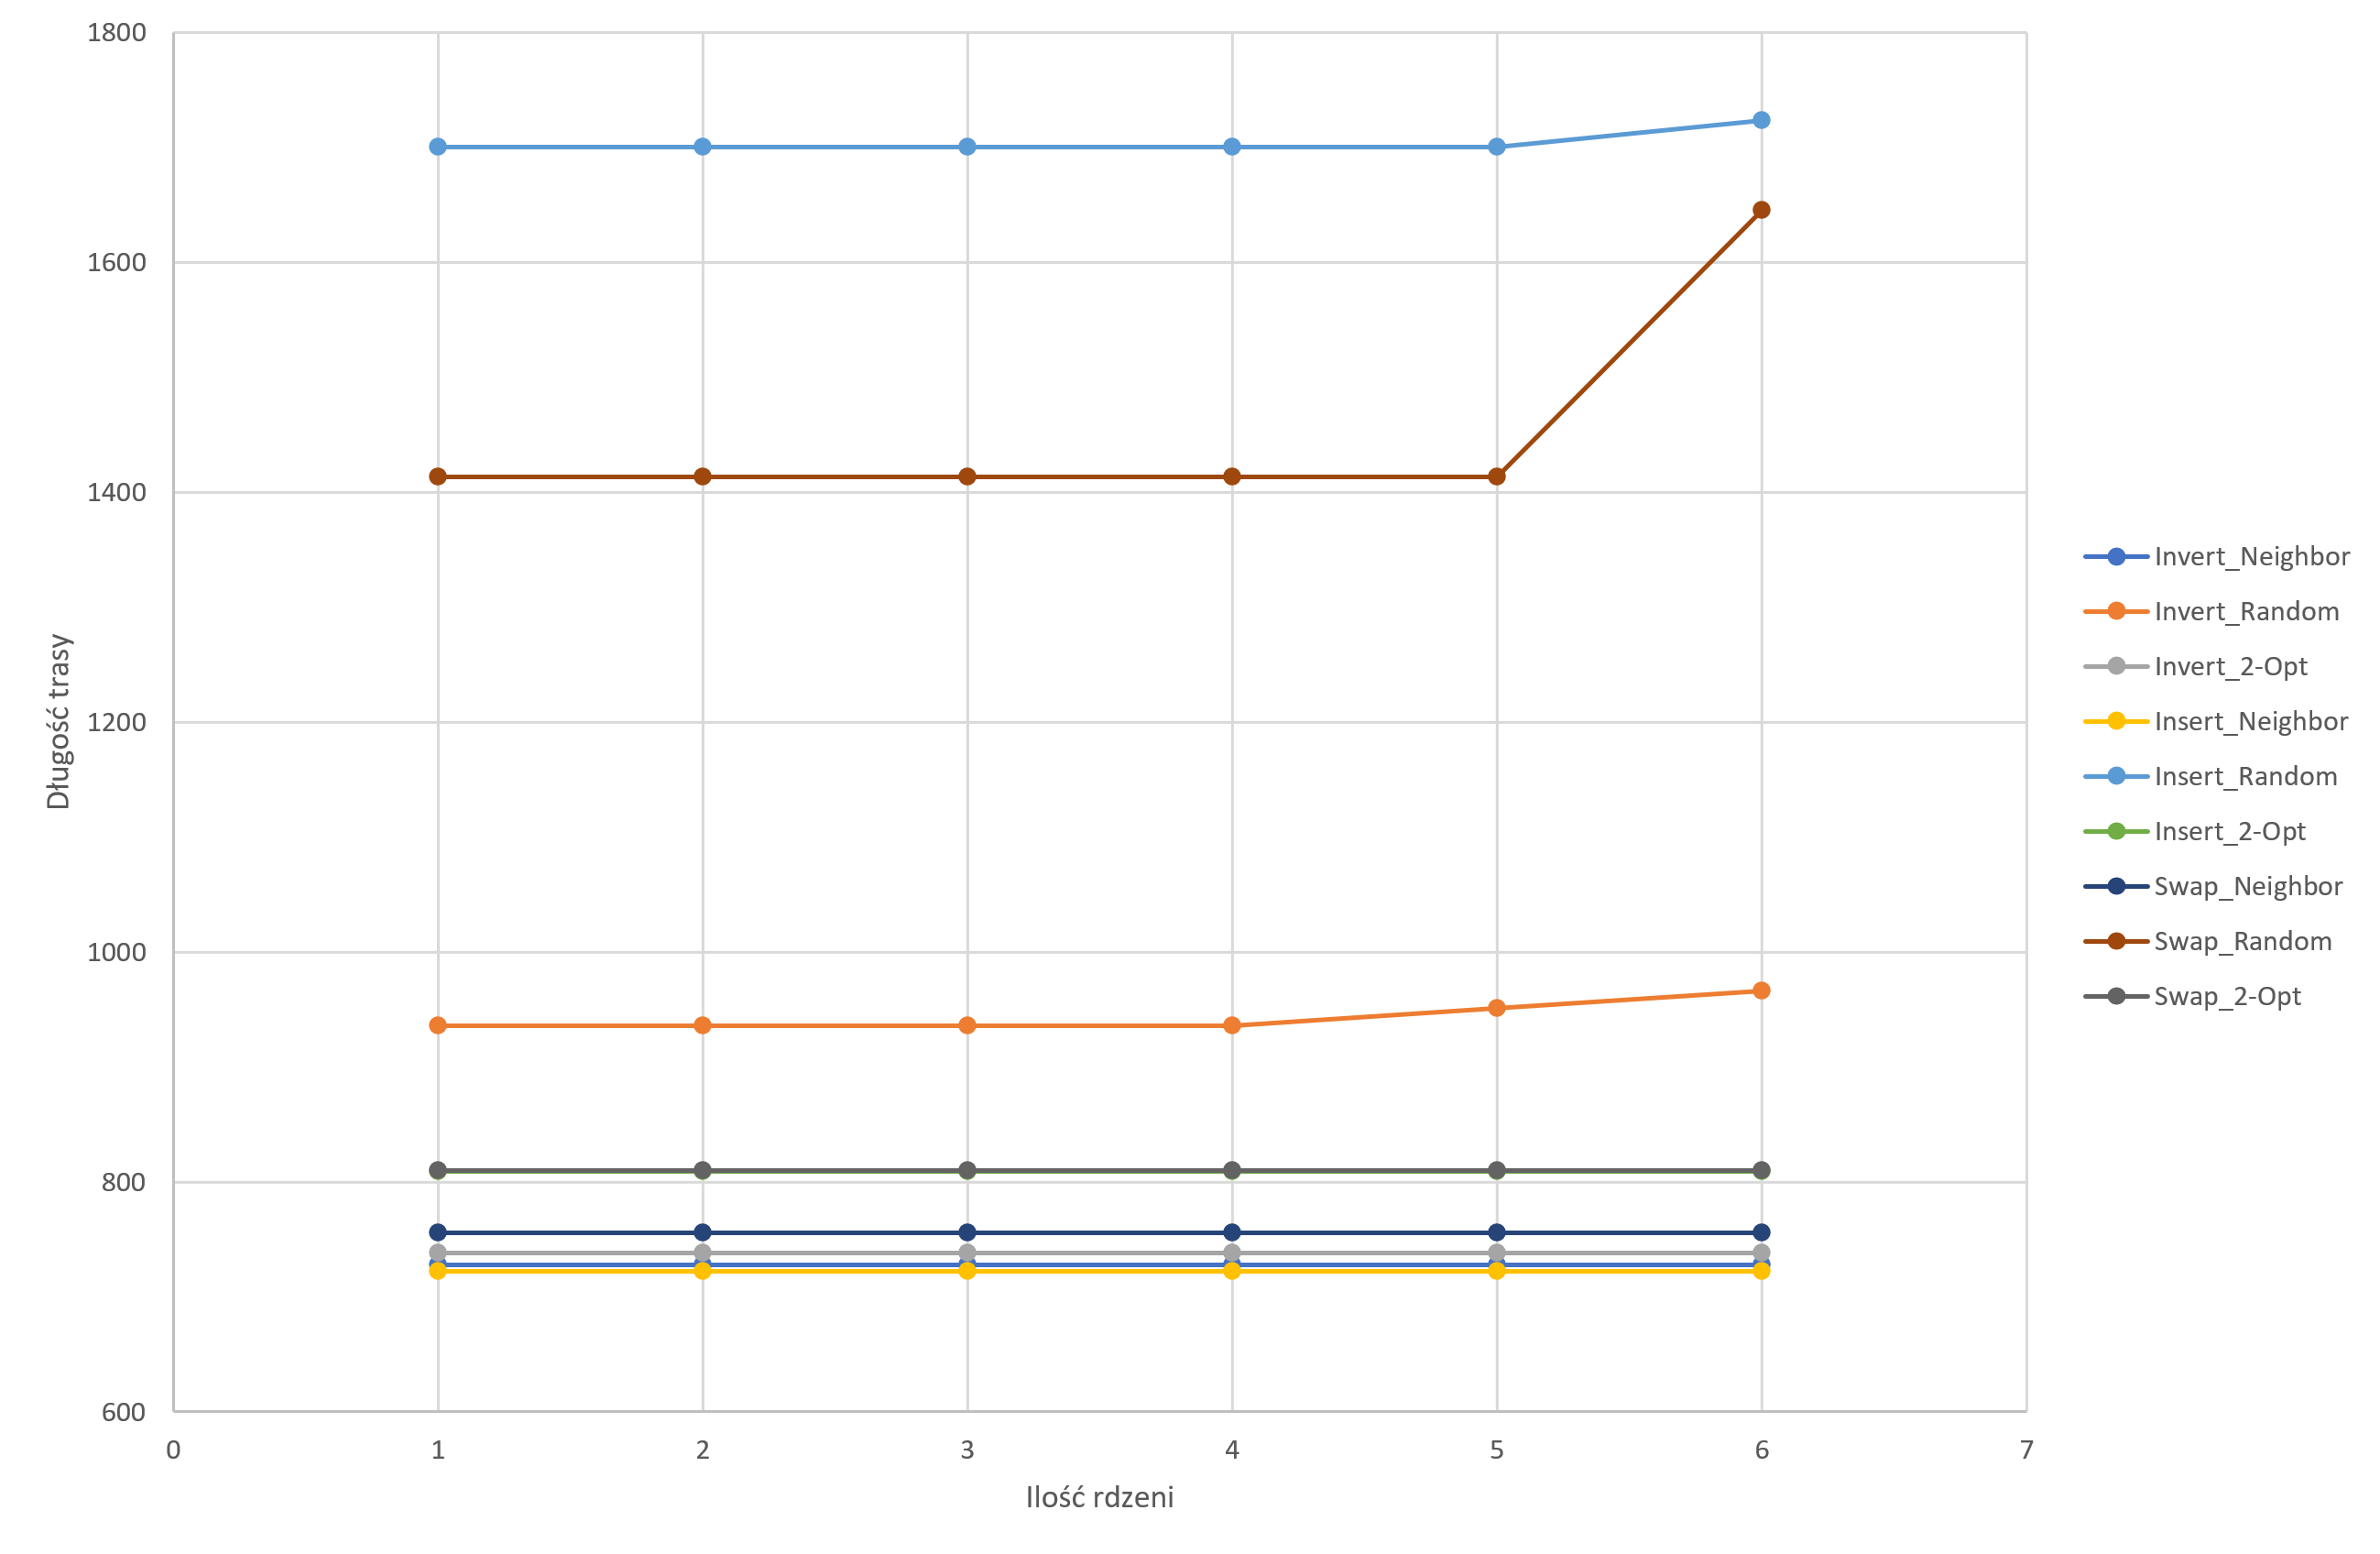
\includegraphics[scale=0.4]{parallel_n=70}

Dla każdego otoczenia i każdego rodzaju trasy startowej nie uzyskano w ten sposób polepszenia trasy.


\end{document}